\documentclass[Master,MSE,german]{twbook}
\usepackage[utf8]{inputenc}
\usepackage[T1]{fontenc}
\newcommand{\FHTWCitationType}{IEEE}
\usepackage{bibgerm}
\usepackage{float}
\usepackage{eurosym}

% Definition Code-Listings Formatierung:
\usepackage[final]{listings}
\lstset{captionpos=b, numberbychapter=false,caption=\lstname,frame=single, numbers=left, stepnumber=1, numbersep=2pt, xleftmargin=15pt, framexleftmargin=15pt, numberstyle=\tiny, tabsize=3, columns=fixed, basicstyle={\fontfamily{pcr}\selectfont\footnotesize}, keywordstyle=\bfseries, commentstyle={\color[gray]{0.33}\itshape}, stringstyle=\color[gray]{0.25}, breaklines, breakatwhitespace, breakautoindent}
\lstloadlanguages{[ANSI]C, C++, [gnu]make, gnuplot, Matlab}

\makeatletter
\renewcommand\lstlistingname{Quellcode}
\renewcommand\lstlistlistingname{Quellcodeverzeichnis}

% Definition des Macros listoflolentryname analog zu listoflofentryname und listoflotentryname der KOMA-Klasse
\newcommand\listoflolentryname\lstlistingname
% Neudefinition der Zeilen des Quellcodeverzeichnisses wenn die Option listof=entryprefix gewählt wurde
\@ifclasswith{scrbook}{listof=entryprefix}
{%
    \renewcommand\l@lstlisting[2]{\@dottedtocline{1}{1.5em}{1em}{\listoflolentryname~#1}{#2}}
}{%
}
\makeatother
\newcommand{\listofcode}{\phantomsection\lstlistoflistings}

%
% Einträge für Deckblatt, Kurzfassung, etc.
%
\title{Erstellung eines Prozesses für die Planungsphase der Softwarearchitektur}
\author{Bernhard Posselt, BSc}
\studentnumber{1310299032}
\supervisor{Mag. Maria-Therese Teichmann}
\place{Wien}
\kurzfassung{Softwarearchitektur ist ein sehr breites Gebiet und sehr abstraktes Gebiet der Softwareentwicklung, ist aber Voraussetzung für qualitativ hochwertige Software. Der hohe Abstraktionsgrad ist aber oft ein Hindernis für eine dem/der KundIn kommunizierbare, reproduzierbare und qualitativ hochwertige Architektur.

Deswegen wird in dieser Arbeit ein reproduzierbarer und kommunizierbarer Architekturerstellungsprozess entworfen. Da laut Zehner-Regel der Fehlerkosten die Behebungskosten unentdeckter Fehler im Laufe des Projektes exponentiell ansteigen, beschränkt sich der Prozess auf die frühe Architekturplanungsphase, um eine möglichst große Wirkung zu erzielen.

Nach mehreren Versuchen, welche wie viele Architekturreviewmethoden stark auf die Priorisierung der Qualitätsmerkmale der Anforderungen aufbauten, wurde jedoch klar, dass sich in der frühen Planungsphase aufgrund der fehlenden Implementation zu wenig messbare Werte für einen reproduzierbaren Prozess ermitteln lassen.

Der Prozess baut daher auf verfügbaren Werten wie Nachbarsystemen, Netzwerken und Risikokosten im Bezug auf unerlaubten Datenzugriff auf. Zusätzlich versucht er durch Analysen der ermittelten Komponentenstruktur Hinweise auf in der Implementationsphase problematische Bereiche zu geben.

Der schließlich erstellte Prozess ist reproduzierbar und die resultierende Architektur aufgrund der Kosten und verwendeten Modellierungssprache UML gut dem/der KundIn kommunizierbar.}
\schlagworte{Softwarearchitektur, Softwareentwicklung, Qualität}
\outline{Software architecture is a very wide and abstract subject in the field of software development but is required to create high quality software. Because of the high grade of abstraction, communicating and creating a reproducible, high quality software architecture is often very hard.

Therefore this thesis will outline a reproducible and communicable software architecture process. Because errors are more costly to fix in a later phase of software development the process itself will focus only on the planing phase in order to achieve high level of effectiveness.

After various attempts to create a software architecture process based on prioritized quality factors which in turn are also often used in many software review processes, it became obvious that there were too few measurable values to create a reproducible process. This was mostly a result of the missing implementation.

The process therefore builds on early available information such as adjacent systems, networks and costs which would be created on unpermitted data access. Additionally the process anaylses the created component structure to reveal possible risk areas which should be closely monitored in the following implementation phase.

The result is a reproducible and, because of its cost based approach and modelling language UML, can be communicated well to the client.}
\keywords{software architecture, software development, quality}

\begin{document}


\maketitle

\chapter{Einführung}

\section{Motivation}


\subsection{Wie kommt man von Anforderungen auf eine gute Architektur}
Vermutung: Gute Architektur häng von guten Anforderungen ab, deswegen muss Anforderungsprozess erweitert werden
Probleme aufzählen die bei einer schlechten Architektur entstehen.

Vermutung: architektur hauptverantwortlich für nicht funktionale Anforderungen, also muss system unter berücksichtigung der nicht funktionalen anforderung erstellt werden

vielleicht noch genauer spezifizieren dass es keine all round solution werden soll sondern die meisten use cases abdecken soll (grafik wieviel apps SOA haben zb)

\subsection{Gibt es eine Art Kochrezept für die Architekturerstellung}
Gesucht: Ein Prozess mit dem auf die wichtigen Faktoren eingegangen werden kann.

\section{Was wird gemacht}
\subsection{Planung einer Zertifizierungsstellen Architektur}
\subsection{Modellierung mit UML}
\subsection{Anpassen der Anforderungestemplates}
\subsection{Architekturplanung Prozesserstellung, eine Art Framework}
\subsection{Dokumentation der Prozesserstellungsanläufe}

\section{Was wird nicht gemacht}
\subsection{Abdeckung des kompletten Prozesses}
Weil zu umfangreich, genauere Beschreibung im Architektur kapitel, auch erklären dass es sich heraus gestellt hat dass man nicht alles sofort planen und bewerten kann wegen fehlenden Messmöglichkeiten
\subsection{Kein Organisations- und Kommunikationsmanagement}
\subsection{Implementation}
Zu umfangreich
\subsection{Abdeckung aller möglichen Architekturfälle (Embedded, High Performance)}
\subsection{Abdeckung aller möglichen Archtekturreviewmethoden}
\subsection{Komplette Vorgaben der Bewertungs-Methoden}
Eher Hinweise auf wie man zb Ausfallkosten bewerten könnte, Methode auf eigene Anwendungsfälle abänder- und ersetzbar. Aber aufzeigen warum es gut sein kann sie dennoch schon zu behandeln
\subsection{Kompletter Anforderungsprozess}
Nur eine Erweiterung im Hinblick auf benötigte Parameter

\section{Übersicht}
Die Arbeit teilt sich in folgende Kapitel auf:

\begin{itemize}
  \item Softwarequalität
  \item Softwarearchitektur
  \item Modellierung in der Architektur
  \item Prozesserstellungsversuche
  \item Ermittlung der Architekturanforderungen
  \item Erstellung der Architektur
  \item Zusammenfassung
\end{itemize}


\subsection{Softwarequalität}
Die Sicherstellung der Softwarequalität ist eines der wichtigsten Ziele bei der Erstellung der Softwarearchitektur, unter Anderem weil die Architektur die Struktur der zu erstellenden Software mitbestimmt und somit gewisse Qualitätsmerkmale begünstigt oder limitiert.

Um dieses Ziel zu verstehen, muss zuerst definiert werden, was Softwarequalität respektive Qualität überhaupt bedeutet. Eine Antwort darauf liefert der in ISO 9126 beschriebene Standard und dessen Nachfolger ISO 25010, auf welchen aber aus geringen Verbreitungsgründen aber nur kurz hingewiesen wird.

ISO 9126 definiert Softwarequalität in der Erfüllung der Anforderungen. Diese lassen sich in funktionale und nicht funktionale Anforderungen aufspalten, wobei bei der Architekturerstellung der primäre Fokus auf den nicht funktionalen Anforderungen liegt.

\subsection{Softwarearchitektur}
Architektur versucht durch Abstraktion die Grundpfeiler der Software fest zu legen. Dies wird standardmäßig durch die Verwendung von Architektursichten erreicht. Es gibt mehrere verschiedene Modelle, welche unterschiedliche Sichten definieren. Um zu erläutern, wie diese Sichten genau verwendet werden können, kann unter Anderem das Modell von Kruchten und das Zachman Framework verwendet werden.

Wie gestaltet sich jedoch der genaue Ablauf der Architekturerstellung? Der Architekturprozess kann in mehrere Abschnitte aufgeteilt werden: Nach einem kurzen Anfangsprozess nach der Anforderungsanalyse kann mit der Planung, Erstellung, Überprüfung der Architektur begonnen werden. Dabei muss auch die Kommunikation beachtet werden.

Für die Überprüfung der Architektur werden Architekturreviewframeworks verwendet. Das Bekannteste unter ihnen ist ATAM, welches durch mehrere Szenarientypen die Qualitätsmerkmale der gewählten Architektur zu überprüfen versucht. Eine weitere Reviewmethode ist CBAM, welche auf ATAM aufbaut aber vor Allem das Preis-Leistungsverhältnis als Entscheidungsgrundlage verwendet.

\subsection{Modellierung in der Architektur}
\subsection{Prozesserstellungsversuche}
\subsection{Ermittlung der Architekturanforderungen}
\subsection{Erstellung der Architektur}
\subsection{Zusammenfassung}
\chapter{Softwarequalität}
Für viele KundInnen ist Softwarearchitektur ein schwer einorden- und erklärbares Teilgebiet der Softwareentwicklung. Deswegen ist es schwierig, den/die KundIn für die Mithilfe an der Architekturerstellung und die daraus resultierenden Kosten zu gewinnen. Eine mögliche Lösung für dieses Problem ist es, die durch unzureichende Softwarequalität entstandenen Kosten, welche wiederum die Folge einer mangelhaften Architektur sind, den Kosten der Architekturerstellung gegenüber zu stellen.  \cite[S. 8-9]{softarch}


Eine gute Softwarearchitektur allein kann zwar nicht eine hohe Softwarequalität garantieren, ist jedoch ein wichtiger Faktor, ohne welchen keine hochqualitative Software erstellt werden kann. Softwarequalität und Softwarearchitektur stehen somit in einem engen Zusammenhang. \cite[S. 8-9]{softarch}

Was genau verbirgt sich jedoch hinter dem Begriff Softwarequalität? Der Begriff Qualität selbst ist sehr breit und schwer definierbar. Laut Garvin gibt es fünf verschiedene Herangehensweisen \cite[S. 25-29]{quality}:

\begin{itemize}
  \item Transzendentale Sicht
  \item Produktbasierte Sicht
  \item Userbasierte Sicht
  \item Herstellungsbasierte Sicht
  \item Wertbasierte Sicht
\end{itemize}

Die transzendentale Sicht beschreibt Qualität als sofort erkennbar, aber als nicht wirklich beschreibbar. Die produktbasierte Sicht ordnet die Qualität des Produktes dessen Bestandteilen zu. Bei der userbasierten Sicht geht es darum, die Anforderungen des/der NutzerInnen zu befriedigen: Die höchste Qualität eines Produktes wird daher erreicht, wenn der/die BenutzerIn alles vorfindet, was er/sie sich erwartet, nicht Mehr und nicht Weniger. Die herstellungsbasierte Sicht misst Qualität an der Erfüllung der Spezifikation und des Designs. Die wertbasierte Sicht schließlich definiert die Qualität durch das Preis-Leistungsverhältnis. \cite[S. 26]{quality}

Diese Sichten treffen mehr oder weniger auch für Softwarequalität zu \cite[S. 399]{pract}, sind aber noch zu grob formuliert, um konkrete Schritte bei der Erstellung des Systems und dessen Architektur zu setzen und konkrete Werte für die Überprüfung der Qualität fest zu legen. Eine genaue Auflistung der für Softwarequalität relevanten Faktoren, bzw. ein Modell, welches den Qualitätsprozess unterstützt, ist somit von Nöten.

\section{Softwarequalitätsmodelle}
ISO 9126 \cite{ISO_SQ} und dessen Nachfolger ISO 25010 \cite{ISO_SQ2} bieten ein Modell, um Softwarequalität zu beschreiben. ISO 25010, der Nachfolgestandard, erweitert die in ISO 9126 beschriebenen Hauptkategorien um Security und Compatibility. Auch die Kategorie Software Quality in Use erfährt eine Überarbeitung: Sie enthält nun die Kategorie Usability, welche vorher in den Hauptkriterien definiert war. Da es aber schwierig war, zitierbare Quellen zum neuen Standard zu finden - ISO 25010 hat \glqq in die Praxis wenig Einzug gehalten\grqq \ \cite[S. 60]{effektiv} - , die Neuerungen überschaubar und mehr eine Umorganisierung als Revolution darstellen, wird auf die Nutzung von ISO 25010 verzichtet und das Qualitätsmodell des Vorgängers, ISO 9216, verwendet.

ISO 9126 definiert folgende Qualitätskategorien:

\begin{itemize}
  \item \glqq Functionality\grqq
  \item \glqq Reliability\grqq
  \item \glqq Usability\grqq
  \item \glqq Efficiency\grqq
  \item \glqq Maintainability\grqq
  \item \glqq Portability\grqq
\end{itemize}


Die beschriebenen Kategorien können laut dem International Requirements Engineering Board, kurz IREB, wiederum in folgende Überkategorien eingeteilt werden: funktionale Anforderungen und nicht funktionale Anforderungen (Abbildung \ref{fig:iso9126}).

\begin{figure}[H]
    \centering
    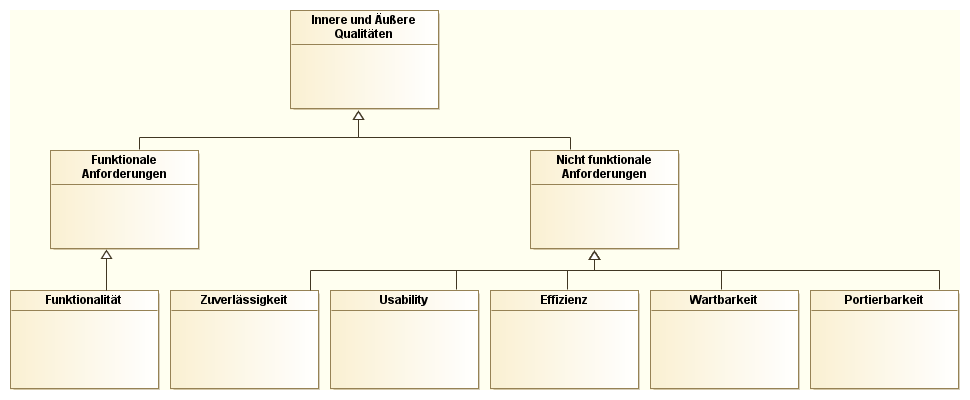
\includegraphics[scale=0.48]{img/iso9126.png}
    \caption{Die Qualitätskategorien des ISO 9126 Standards unterteilt in funktionale und nicht funktionale Anforderungen}
    \label{fig:iso9126}
\end{figure}


\section{Funktionale Anforderungen}
Funktionale Anforderungen beschreiben die Funktionalität des Systems, welche die Geschäftsprozesse des/der KundIn umsetzen und das System für ihn/sie somit wertvoll machen \cite[S. 79]{reqanalysis}. Sie werden vom/von der KundIn meist in der Form von Usecases beschrieben \cite[S. 78]{reqanalysis}

IREB ordnet die Functionality Kategorie von ISO 9126 den funktionalen Anforderungen zu\cite[S. 9]{ireb}, welche sich in folgende Unterkategorien aufspaltet:

\begin{itemize}
  \item \glqq Suitability\grqq
  \item \glqq Accuracy\grqq
  \item \glqq Interoperability\grqq
  \item \glqq Security\grqq
  \item \glqq Functional compliance\grqq
\end{itemize}

Suitability beschreibt das Vorhandensein von Funktionen, welche die vom/von der NutzerIn geforderten Funktionalitäten bereitstellen. Accuracy behandelt die geforderte Genauigkeit der implementierten Funktionen, Interoperability wiederum die Interaktionsmöglichkeiten des Systems mit anderen Systemen. Security beschreibt die implementierten Kontroll- und Sicherheitsmechanismen, mit welchen das System die Daten vor unerlaubtem Zugriff schützt. Der letzte Punkt, Functional Compliance, beschreibt die Standard- und Gesetzeskonformität des Softwareprodukts. \cite[S. 8]{ISO_SQ}

\section{Nicht funktionale Anforderungen}
Nicht funktionalen Anforderungen \glqq verkörpern Erwartungen und Notwendigkeiten, die von Interessensvertretern (Auftraggeber, Benutzer, Architekt, Entwickler, etc.) neben den funktionalen Anforderungen als wichtig erachtet werden und über die reine gewünschte Funktionalität hinausgehen\grqq \cite[S. 108]{softarch}. Sie definieren nicht das Was sondern das Wie \cite[S. 80]{reqanalysis}.

Der Fokus liegt meist auf der Funktionalität eines Systems; es ist schließlich der Hauptgrund für die Erstellung des Systems und der/die KundIn hat eine genaue Vorstellung, was das System genau können muss. Die Qualität des Systems ist meist eine implizite Anforderung, welche im Anforderungsprozess besonders beachtet werden muss, aber trotzdem essentiell für den Erfolg des Systems ist. \cite[S. 109]{softarch}

Dies lässt an folgendem Beispiel demonstrieren: Ein/Eine KundIn beauftragt eine Firma, einen Webshop zu erstellen, auf welchem er/sie seine/ihre Produkte verkaufen will. Die Funktionalität des Webshops wird wie beschrieben implementiert, aber das Endprodukt ist so langsam, dass ein Großteil der KundInnen den Bestellvorgang abbricht. Der Hauptfunktion des Systems, nämlich Produkte verkaufen, ist somit zwar prinzipiell möglich, aber für den/die KundIn im Vergleich zur investierten Summe unrentabel.

Nicht funktionale Anforderungen sind nicht nur oft implizite Anforderungen, sondern auch schwer bezifferbar: Oft wird zB. einfach verlangt, dass das System schnell sein soll. Eine genaue Definition, was der/die KundIn unter schnell versteht ist schwer zu ermitteln. Außerdem sind durch die Kontextabhängigkeit des Begriffes keine allgemeingültigen Werte ermittelbar: Eine ein Sekunden lange Antwortzeit kann für die Nutzung einer Buchhaltungssoftware schnell genug sein, werden die Daten aber für zeitkritische Anwendungen wie Aktienkäufe benötigt, ist die selbe Antwortzeit inakzeptabel. \cite[S. 59]{effektiv}.

Es sind jedoch besonders die nicht funktionalen Anforderungen, welche im Fokus der Architekturerstellung liegen: Durch die in der Architekturphase entwickelte Struktur der Applikation wird die Erfüllung bestimmter Qualitätsmerkmale überhaupt erst möglich. Die Architektur beinflusst somit die nicht funktionalen Qualitäten eines Systems stark \cite[S. 109]{softarch}. Dies erlaubt folgenden Umkehrschluss: \glqq Architektur ist für die Qualität eines Systems notwendig\grqq \cite[S. 59]{effektiv}. \cite[S. 19]{effektiv}

Weil die Qualität des Systems wie beschrieben maßgeblich von der Architektur abhängt, welche wiederum von den Qualitätsmerkmalen nicht funktionaler Anforderungen abhängt, ist auch die Ermittlung, Korrektheit und Präzision dieser Anforderung für die Architektur von hoher Bedeutung.

Die nicht funktionalen Anforderungen in ISO 9126 werden vom IREB den  verbleibenden Kategorien zugeschrieben. Darunter fallen folgende Kategorien\cite[S. 9]{ireb}:

\begin{itemize}
  \item \glqq Suitability\grqq
  \item \glqq Accuracy\grqq
  \item \glqq Interoperability\grqq
  \item \glqq Security\grqq
  \item \glqq Functional compliance\grqq
\end{itemize}

All diese Kategorien haben wie die Functionality Kategorie eigene Unterpunkte.

\subsection{Reliability}
Die Reliability Kategorie beschreibt die Zuverlässigkeit des Systems unter Last und besteht aus folgenden Unterpunkten \cite[S. 7]{ISO_SQ}:

\begin{itemize}
  \item \glqq Maturity\grqq
  \item \glqq Fault tolerance\grqq
  \item \glqq Recoverability\grqq
  \item \glqq Reliability compliance\grqq
\end{itemize}

Maturity beschreibt die Fähigkeit des Systems, Ausfälle des Systems wegen Softwarefehlern zu vermeiden; Fault Tolerance wiederum behandelt die Fähigkeit des Systems eine gewisse Leistung des Systems trotz Softwarefehler zu ermöglichen. Recoverability beschreibt Fähigkeiten eines Systems  sich von Fehlern zu erholen. Reliability Compliance bezieht sich auf die Konformität gegenüber Standards und Konventionen. \cite[S. 8-9]{ISO_SQ}

\subsection{Usability}
Die Usability Kategorie beschreibt die Benutzbarkeit des Systems und besteht aus folgenden Unterpunkten \cite[S. 7]{ISO_SQ}:

\begin{itemize}
  \item \glqq Understandability\grqq
  \item \glqq Learnability\grqq
  \item \glqq Operability\grqq
  \item \glqq Attractiveness\grqq
  \item \glqq Usability compliance\grqq
\end{itemize}

Understandability beschreibt die Einfachheit, mit welcher ein/eine BenutzerIn das System für eine bestimmte Aufgabe als verwendbar klassifiziert, Learnability beschreibt, wie leicht ein/eine BenutzerIn das System erlernen kann. Operability beschreibt, in wieweit ein/eine BenutzerIn das System bedienen und kontrollieren kann. Actractiveness beschreibt, ob das Aussehen von den NutzerInnen als attraktiv wahrgenommen wird. Usability Compliance schließlich beschreibt die Konformität gegenüber Standards, Styleguides und Konventionen. \cite[S. 9-10]{ISO_SQ}

\subsection{Efficiency}
Die Efficiency Kategorie umschreibt den Leistungs- und Resourcenhunger eines Systems und besteht aus folgenden Unterpunkten \cite[S. 7]{ISO_SQ}:

\begin{itemize}
  \item \glqq Time behaviour\grqq
  \item \glqq Resource utilisation\grqq
  \item \glqq Efficiency compliance\grqq
\end{itemize}

Time Behavior beschreibt die Antwort-, Rechenzeiten und die Durchsatzraten des Systems. Resource Utilisation umfasst die Typen und den Verbrauch von Resourcen. Efficiency Compliance bezieht sich wiederum um die Standard- und Konventionskonformität des Systems. \cite[S. 10]{ISO_SQ}

\subsection{Maintainability}
Die Maintainability Kategorie beschreibt, wie einfach ein System gewartet und modifziert werden kann und besteht aus folgenden Unterpunkten \cite[S. 7]{ISO_SQ}:

\begin{itemize}
  \item \glqq Analysability\grqq
  \item \glqq Changeability\grqq
  \item \glqq Stability\grqq
  \item \glqq Testability\grqq
  \item \glqq Maintainability compliance\grqq
\end{itemize}

Analysability beschreibt, wie einfach ein System nach Fehlern oder Problemen untersucht werden kann, Changeability wie einfach es ist, Änderungen durchzuführen. Stability besagt, wie wahrscheinlich es ist, dass nach einer Änderung unvorhergesehene Probleme auftreten, Testability wie schwer es ist, das System zu testen. Maintainability compliance, wie auch in den vorherigen Fällen, beschreibt die Standardkonformität. \cite[S. 10-11]{ISO_SQ}


\subsection{Portability}
Die Portability Kategorie beschreibt, wie einfach der Wechsel auf andere Hardware- und Softwareumgebungen möglich ist und besteht aus folgenden Unterpunkten \cite[S. 7]{ISO_SQ}:

\begin{itemize}
  \item \glqq Adaptability\grqq
  \item \glqq Installability\grqq
  \item \glqq Co-existence\grqq
  \item \glqq Replaceability\grqq
  \item \glqq Portability compliance\grqq
\end{itemize}

Adaptability behandelt die Anpassungsfähigkeit an andere Umgebungen, zB. verschiedene Displaygrößen. Installability befasst sich mit der Einfachheit der Installation.  Co-existence beschreibt, wie sich das Programm gegenüber anderen, auf dem gleichen System laufenden Programmen verhält,   Replaceability in wieweit das System durch ein anderes ersetzt werden kann. Portability compliance behandelt abschließend die Standardkonformität. \cite[S. 11]{ISO_SQ}
\chapter{Softwarearchitektur}
Softwarearchitektur beschäftigt sich mit dem Erstellen des Fundamentes eines Softwareprojektes \cite[S. 9]{softarch}. Der Fokus liegt daher nicht auf Implementationsdetails sondern auf Schnittstellen, welche das System und die Zusammenarbeit der Teilkomponenten beschreiben \cite[S. 8]{basiswissen}. Ziel der Softwarearchitektur ist es, durch Abstraktion der Details einen Überblick über die zu implementierenden Komponenten zu gewinnnen, welcher es ermöglicht, frühe Entscheidungen über die Probleme und Angemessenheit des Systems zu erlangen und somit Risiken, Fehler- und Änderungskosten zu vermeiden oder zu verringern \cite[S. 10]{softarch}.

\section{Architektursichten}
Der Detailgrad der Schnittstellen hängt wesentlich von der Größe des Projektes ab \cite[S. 7-12]{basiswissen}. Um die Komplexität und Abstraktion zu beherrschen, können Architektursichten verwendet werden, welche einen Überblick über Teilbereiche des Systems ermöglichen \cite{ISO_ARCH}. Ein Beispiel dafür ist Kruchtens 4+1 Sichtenmodell \cite{kruch}, welches folgende Sichten beschreibt:

\begin{itemize}
  \item Logical View: Logische Sicht auf das System, welches die Klassen und deren Beziehungen untereinander darstellt
  \item Process View: Beschäftigt sich mit nicht funktionalen Anforderungen wie Performance und Fehlertolleranz und deren Implementierung
  \item Development View: Beschreibt die Aufteilung des Systems in Module und Bibliotheken
  \item Physical View: Regelt und beschreibt die Verteilung der Komponenten auf physische Systeme
  \item Scenarios: Usecases, welche die Nutzung des Systems beschreiben
\end{itemize}

Kruchten verwendet eigene Diagramme für jede Sicht, die an UML angelehnt aber zum Teil verschieden sind, etablierte sich UML doch erst zwei Jahre später nach der Veröffentlichung seines Modelles \cite{glasklar}[S. 5].

Es gibt noch viele andere Sichtenmodelle wie das Zachman Framework \cite[S. 282]{zachman}, welches eine Aufteilung in Kontext-, Geschäfts, System, Technologie, Integrations und Laufzeitsicht vornimmt. Die Gemeinsamkeit aller Sichtenmodelle ist jedoch der Versuch, durch unterschiedliche Sichtweisen einen besseren Überblick über das Zielsystem zu erlangen.



\section{Architekturprozess Lifecycle}
Zeitlich ordnet sich die Architekturphase zwischen dem Ermitteln der Anforderungen und der tatsächlichen Implementation ein. Da die Erstellung von Software heutzutage mehr ein agiler und inkrementeller Prozess ist, wird auch die Erstellung und die Mitwirkung der Softwarearchitektur in diese sich wiederholenden Prozesse mit einbezogen. \cite[S. 7]{basiswissen}

Der Architekturzyklus lässt sich mit dem in Abbildung \ref{fig:cycle} beschriebenen Aktivitätsdiagramm darstellen und unterteilt sich in folgende Unterbereiche \cite[Umschlag]{softarch}:

\begin{itemize}
  \item \glqq Erstellen der Systemvision\grqq
  \item \glqq Verstehen der Anforderungen\grqq
  \item \glqq Entwerfen der Architektur\grqq
  \item \glqq Umsetzen der Architektur\grqq
  \item \glqq Kommunizieren der Architektur\grqq
\end{itemize}


\begin{figure}[H]
    \centering
    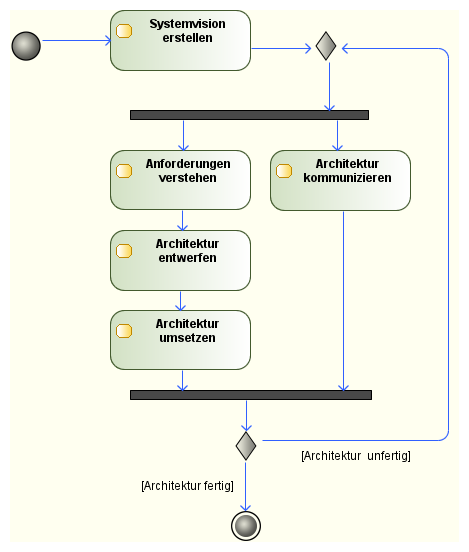
\includegraphics[scale=0.8]{img/archcycle.png}
    \caption{Der Architekturprozess modelliert als Aktivitätsdiagramm \cite[Umschlag]{softarch}}
    \label{fig:cycle}
\end{figure}

Der Fokus der Arbeit liegt wegen der fehlenden Implementierung hauptsächlich auf den ersten drei Teilen, der Erstellung der Systemvision, Verstehen der Anforderungen und dem Entwerfen der Architektur.

\section{Was macht eine gute Softwarearchitektur aus}
Die Frage, was eine gute Softwarearchitektur ausmacht, wird oft sehr breit und ungenau beantwortet: Eine gute Architektur erfülle die \glqq Verhaltens-, Qualitäts- und Lebenszyklusanforderungen\grqq \ \cite[S. 12]{basiswissen} eine Systems, ermögliche es Risiken frühzeitig zu erkennen und die inhärente Komplexität eines Systems und dessen Quellcodes zu beherrschen \cite[S. 7-8]{softarch}.

Alle diese Kriterien lassen sich jedoch schwierig oder gar nicht messen. Manche Werte sind zwar messbar, aber lassen keine eindeutigen Entscheidungen ableiten: zB. können Kopplung und Kohäsion eines Systemes gemssen werden, jedoch kann nicht eindeutig festgelegt werden, ab welchem Wert die Kopplung zu hoch oder die Kohäsion zu niedrig ist.

Dieter Masek kommt zu folgendem Schluss: \glqq Die Frage ob eine gegebene Architektur gut oder schlecht ist, lässt sich nicht direkt beantworten. Gut oder schlecht sind absolute Bewertungen, die für Architekturen sowieso nicht möglich sind. Eine Architektur lässt sich nur in einem festgelegten Kontext beurteilen d.h.: Wie gut löst eine Architektur ein vorgegebenes Problem? Selbst diese eingeschränkte Frage lässt sich nicht mit gut oder schlecht beantworten! \grqq \ \cite[S. 19]{review}

Trotz all dieser Probleme lassen sich dennoch Werte messen und überprüfen \cite[S. 19]{review}, welche in Verbindung mit unzureichenden Architektureintscheidungen gebracht werden können. Dies erlaubt folgenden Schluss: Die Ausgangsfrage, was eine gute Softwarearchitektur ausmacht, führt zu keiner Erkenntnis und ist damit mehr oder minder nutzlos: Es kommt nicht darauf an, ob eine Architektur gut ist, sondern ob eine Architektur die an sie gestellten Anforderungen erfüllt.

Viele dieser Anforderungen stehen im Gegensatz zueinander: zB. erfordert eine hohe Performance eine niedrigere Abstraktionsebene, was jedoch die Wartung des Codes erschwert. Die Findung einer angemessene Softwarearchitektur beschäftigt sich somit mehr mit der Abwägung von Vor- und Nachteilen, welche aus den jeweiligen Entwurfsmustern und Technologien ableitbar sind.

Um diese Entscheidungen abwägen zu können, ist wichtig, die expliziten Anforderungen an das System zu kennen \cite[S. 19]{review}. Eine möglichst vollständige Anforderungsanalyse ist somit die Ausgangsbasis für eine angemessene Softwarearchitektur. Dies kann jedoch vor allem am Anfang der Anforderungsanalyse schwierig sein, da die KundInnen noch keine genaue Vorstellung vom zu entwickelnden System haben \cite[S. 80]{reqman}.

Eine Möglichkeit zur Überprüfung von bestehenden und noch nicht beachteteten Anforderungen der Architektur stellt die Durchführung eines szenariobasierten Architekturreviews wie ATAM oder CBAM dar.


\section{Architekturbewertungsmethoden}
Kurze Einführung in Architekturbewertungsmethoden

\subsection{ATAM}
\subsection{CBAM}
\chapter{Modellierung in der Architektur}
Der Architekturprozess \glqq erstreckt sich von der Analyse des Problembereichs eines Systems bis hin zu seiner Realisierung\grqq \cite[S. 10]{softarch} und arbeitet durch die verschiedenen Architektursichten stark mit verschiedenen Mitteln der Abstraktion. Wien in ISO 42010 beschrieben besitzt jede Architektursicht zudem ein oder mehrere Architekturmodelle \cite{ISO_ARCH}. Werden Architektursichten im Architekturprozess verwendet, bietet sich deswegen auch die Verwendung von Modellierungssprachen an, mit welchen die Architekturmodelle erstellt werden können.

\section{Modelldefinition}
Ein Modell hat laut Stachowiak folgende Eigenschaften \cite[S. 131-133]{modell}:

\begin{itemize}
  \item Abbildung
  \item Verkürzung
  \item Pragmatismus
\end{itemize}

Das Abbildungsmerkmal besagt, dass Modelle entweder natürliche oder künstliche Dinge abbilden. Das Verkürzungsmerkmal eines Modells dreht sich um die Reduktion der Eigenschaften des Originals: Nur die für den Einsatzbereich relevanten Eigenschaften werden durch das Modell repräsentiert. Das Pragmatismusmerkmal schließlich besagt, dass Modelle eine Funktion erfüllen: Sie sind sowohl für einen definierten Einsatzzweck, als auch für eine Person, sei sie natürlich oder künstlich, erstellt. \cite[S. 131-133]{modell}

Werden Modelle verwendet, müssen diese kommuniziert und dokumentiert werden \cite[S. 12]{reqanalysis}. Vor Allem in der Arbeit im Team bietet sich deswegen eine standardisierte Modellierungssprache an, welche den Einsatzbereich so gut wie möglich abdeckt. Dies dient vor Allem dazu, Interpretationsfehler zu vermeiden. Aus dem gleichen Grund ist es auch vorteilhaft, eine weit verbreitete Modellierungssprache zu wählen \cite[S. 139]{effektiv}. Eine Modellierungssprache sollte zudem visuelle Elemente verwenden, da das menschliche Auge Bilder schneller als Text aufnehmen kann \cite[S. 12]{reqanalysis}.

\section{UML}
UML, kurz für Unified Modelling Language, ist eine in den 90ern entstandene Modellierungssprache, welche sich vor Allem für die Modellierung objektorientierter Systeme eignet \cite[S. 145]{basiswissen}. Sie war eine Antwort auf den damaligen Wildwuchs an verschiedenen, zueinander inkompatiblen Modellierungssprachen wie OOD, OOA\&D, etc. \cite[S. 5]{glasklar}. Mittlerweile ist sie weit verbreitet und wird weltweit verstanden \cite[S. 138]{effektiv}. Die aktuelle Version der UML ist 2.4.1 \cite{omg}.


Die in der UML spezifizierten Diagramme lassen sich in folgende zwei Kategorien einteilen \cite[S. 105, 239]{glasklar}\cite[S. 146]{basiswissen}:

\begin{itemize}
  \item Verhaltensdiagramme
  \item Strukturdiagramme
\end{itemize}

UML Diagramme lassen sich im Architekturprozess vor Allem zur Beschreibung der verschiedenen Architektursichten einsetzen und bieten alle für die Abstraktion des Systems im Architekturprozesses benötigten Werkzeuge\cite[S. 139]{effektiv}. Durch ihre verkürzende Wirkung und höhere Informationsdichte sind UML Diagramme auch oft Artefakte des Anforderungsprozesses \cite[S. 215]{reqman}. UML schlägt somit die Brücke vom Anforderungs- zum Architekturprozess. Nicht alle verfügbaren UML Diagramme sind jedoch für die Erstellung und Modellierung der Architektur nötig. \cite[S. 144]{basiswissen}

Die in der Arbeit verwendeten Verhaltensdiagramme beschränken sich auf das Usecase-, Kontext-, Komponenten- und Aktivitätsdiagramm. Das einzig verwendete Strukturdiagramm ist das Klassendiagramm.


\subsection{Usecasediagramm}
Das Usecasediagramm gliedert sich in die Diagrammkategorie der Verhaltensmodellierung ein und beschreibt die Anwendungsfälle des Systems, dessen AkteurInnen und die Beziehung zwischen den Beiden. Die einzelnen Anwendungsfälle selbst repräsentieren Aktionen. Diese werden jedoch nicht im Usecasediagramm modelliert.\cite[S. 242-245]{glasklar}

\begin{figure}[H]
    \centering
    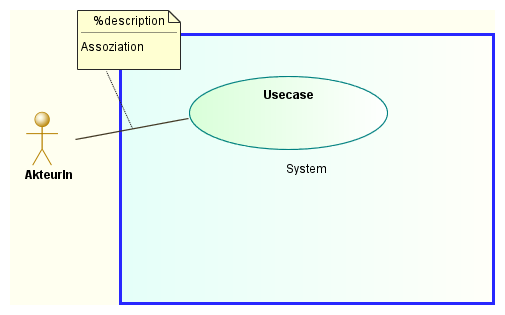
\includegraphics[scale=0.8]{uml/modelling/usecase.png}
    \caption{Das UML Usecasediagramm}
    \label{fig:umlusecasemodel}
\end{figure}

Das Usecasediagramm ist kein Artefakt der Architekturerstellung, sondern wird in der Regel in der Anforderungsanalyse des Projektes erstellt. In der Architekturphase gibt das Diagramm aber Auskunft über wichtige architekturentscheidende Parameter, wie zB. die Systemabgrenzung, Nachbarsysteme, BenutzerInnen und Grundfunktionalität des Systems. Außerdem wird es für Architekturreviewmethoden wie ATAM benötigt und kommt in der Usecase Sicht von Kruchtens 4+1 Modell vor \cite[S. 148]{basiswissen}

\subsection{Kontextdiagramm}
Das Kontextdiagramm kann in die Strukturmodellierung eingeordnet werden und zeigt die AkteurInnen, Datenflüsse und Nachbarsysteme. Das Kontextdiagramm selbst ist nicht Teil der UML, kann aber mit UML dargestellt werden. Meistens wird dafür ein Usecasediagramm verwendet, aber auch ein Komponentendiagramm stellt im Prinzip die notwendigen Elemente bereit. \cite[S. 255]{glasklar}

\begin{figure}[H]
    \centering
    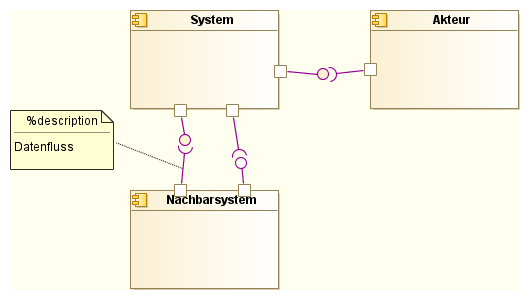
\includegraphics[scale=0.8]{uml/modelling/context.png}
    \caption{Das Kontextdiagramm, dargestellt mit Hilfe des Komponentendiagramms}
    \label{fig:umlcontextmodel}
\end{figure}

Das Kontextdiagramm wird in der Anforderungsanalyse erstellt und gibt einen genaueren Überblick über die Systemabgrenzung \cite[S. 255]{glasklar}. Da es zudem auch die Nachbarsysteme modelliert kann es als Grundstein für die Planung der Komponenten der Architektur herangezogen werden.


\subsection{Komponentendiagram}
Das Komponentendiagramm ist Teil der Strukturdiagramme und wird verwendet, um die Bestandteile eines Systems zu modellieren. Die Implementation der einzelnen Bestandteile, auch Komponenten genannt, wird dabei nicht dargestellt. Stattdessen werden die Schnittstellen der Komponenten und deren Beziehungen untereinander modelliert. Die Komponenten selbst können in Artefakte gekapselt werden. \cite[S. 216]{glasklar}

\begin{figure}[H]
    \centering
    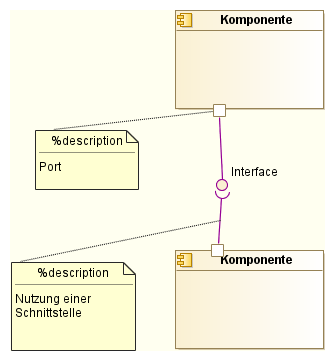
\includegraphics[scale=0.8]{uml/modelling/component.png}
    \caption{Das UML Komponentendiagramm}
    \label{fig:umlcomponentmodel}
\end{figure}

Das Komponentendiagramm modelliert im Gegensatz zum Paketdiagramm bis zu einem gewissen Grad die tatsächliche, physische Aufteilung des Systems und kann in der Architekturplanung deswegen für die Physische bzw. Verteilungssicht verwendet werden \cite[S. 223]{glasklar}\cite[S. 139]{basiswissen}. Durch die Verwendung von Interfaces ermöglicht es eine grobe und frühe Übersicht über das Zusammenspiel des zu entwickelnden Systems.

\subsection{Klassendiagramm}
Das Klassendiagramm fügt sich in die Strukturdiagramme ein und modelliert die Daten, Methoden und deren Beziehungen untereinander. Es kann als Basis für die Erstellung der Datenbanktabellen verwendet werden und übernimmt somit immer öfter die Aufgaben, welche früher dem ER Diagramm zukamen. Eine weitere Aufgabe des Klassendiagramms ist die Modellierung von Interfaces. \cite[S. 108-110]{glasklar}

\begin{figure}[H]
    \centering
    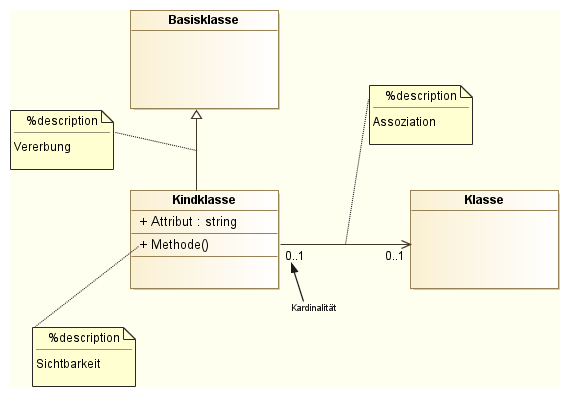
\includegraphics[scale=0.8]{uml/modelling/class.png}
    \caption{Das UML Klassendiagramm}
    \label{fig:umlclassmodel}
\end{figure}


Da die Daten und Interfaces, welche das Klassendiagramm beschreibt, auch in anderen Diagrammen referenziert werden, sind sie ein wichtiger Teil der Architekturerstellung: Interfacediagramme werden für die Beschreibung der Schnittstellen von Komponenten benötigt, Klassendiagramme werden unter Anderem in den Objektflüssen der Aktivitätsdiagramme referenziert. Außerdem lassen sich die Daten für den/die KundIn mit einem Wert beziffern, da die Vertrautheit der Daten durch Gesetze vorgeschrieben sein kann und auch ihr Verlust, Manipulation oder Diebstahl meist finanzielle Folgen nach sich zieht.


\subsection{Aktivitätsdiagramm}
Das Aktivitätsdiagramm wird in die Verhaltensmodellierung eingeteilt und erlaubt es, Abläufe des Systems zu modellieren. Es besteht aus Aktionen, Objektknoten, Kontrollelementen und Kanten, welche die Elemente untereinander verbinden \cite[S. 264]{glasklar}. Durch Objektflüsse und Swimlanes lässt sich der Austausch von Daten zwischen verschiedenen Systemen modellieren. \cite[S. 268]{glasklar}. Diese Flüsse können auch als Nachrichten im Sequenzdiagramm modelliert werden. Das Sequenzdiagramm ist aber zeitraubender zu modellieren, was dazu führt, dass die Wartung oft vernachlässigt wird \cite[S. 414]{glasklar}. \cite[S. 263-274]{glasklar}


\begin{figure}[H]
    \centering
    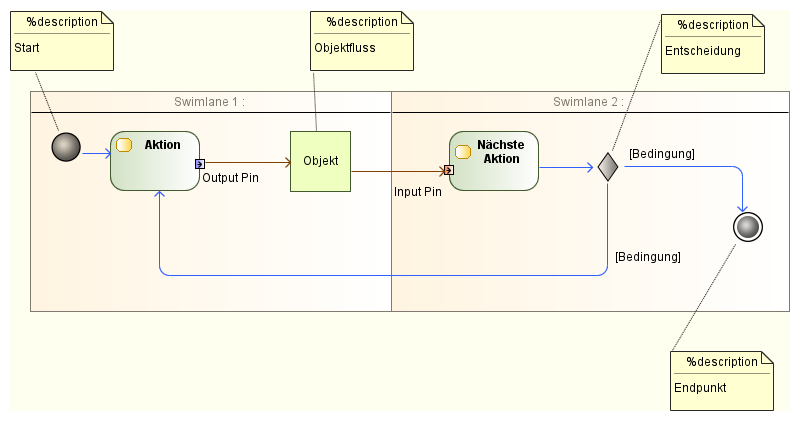
\includegraphics[scale=0.6]{uml/modelling/activity.png}
    \caption{Das UML Aktivitätsdiagramm}
    \label{fig:umlactivitymodel}
\end{figure}


Da sich das Aktivitätsdiagramm vor Allem zur Beschreibung von Businessprozessen und Usecases eignet, ist es bei der Architekturerstellung vor Allem für das Verständnis des Usecasediagrammes wichtig \cite[S. 271-272]{glasklar}. Zusätzlich helfen die modellierten Objektflüsse und Swimlanes bei der Erstellung der Komponenteninterfaces.
\chapter{Prozesserstellungsversuche}
Der Architekturprozess ist komplex und ein falsches Vorgehen kann der Ursprung vieler Probleme sein \cite[S. 7-8]{softarch}. Deswegen ist es notwendig einen eigenen Prozess zu definieren, welcher die Erstellung vereinfacht und die Fehlerkosten minimiert. Dieser Prozess sollte schon in der Planungsphase zum Einsatz kommen, da hier wegen der Zehner-Regel der Fehlerkosten der größte Effekt zur Reduzierung der Fehlerkosten erzielt werden kann \cite[S. 154]{fehler}.

Der Prozess wurde anhand eines Beispielprojektes erstellt und dreht sich um die Architektur eines Systems einer Personenzertifizierungsstelle.

\section{Vorhandene Daten}
Ausgegangen wurde von folgenden Anforderungsdokumenten, welche in der Erstellung des Prozesses mehrfach abgeändert und an die Architekturprozessanforderungen angepasst wurden:

\begin{itemize}
  \item Usecasediagramm: modelliert die Usecases des Unternehmens
  \item Usecasebeschreibung: ausgefülltes Anforderungstemplate, welches Sonderfälle, nicht funktionale Parameter und weitere Details beinhaltet
  \item Klassendiagramm: visualisiert die zu verwendeten Daten
  \item Aktivitätsdiagramme: visualisiert den Ablauf komplexerer Usecases
  \item Kontextdiagramm: zeigt die Datenflüsse zwischen AkteurInnen, Nachbarsystemen und dem zu erstellenden System
  \item ISO Anforderungsdokument für Personenzertifizierungsstellen \cite{ISO_CERT}: beschreibt die Rahmenbedingungen für den Betrieb einer Personenzertifizierungsstelle
\end{itemize}

\section{Prozesserstellungsversuche}
Ausgehend von den vorhandenen Daten wurden mehrere Prozesse definiert, welche bis auf den Letzten entweder zu grobe Ergebnisse lieferten, oder nicht nachvollziehbar waren.

Ausgangsbasis war eine Systemvision mit folgenden Anforderungen:

\begin{itemize}
  \item Es soll eine Webseite entstehen, welche die Prüfungstermine auflistet und Personen erlaubt, sich für diese Prüfungen anzumelden. Dadurch soll der Verwaltungsaufwand reduziert werden, um Kosten zu sparen.
  \item Die Übermittlung der Prüfungsdaten soll über einen eigenen VPN Server geschehen, um die Datensicherheit des Systems zu erhöhen.
  \item Die Prüfungsdaten werden firmenintern verwaltet und nach der Auswertung soll der Scheme Owner benachrichtigt werden. Beide Usecases sollen auf eine sichere Art und Weise umgesetzt werden.
\end{itemize}

\begin{figure}[!htbp]
    \centering
    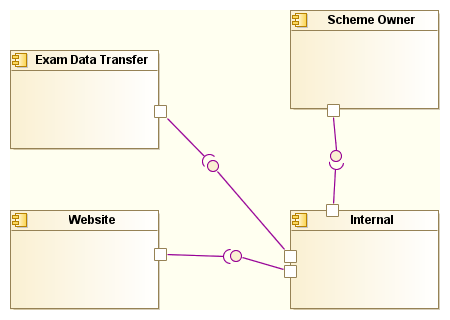
\includegraphics[scale=0.6]{uml/vision.png}
    \caption{Systemvision der Komponenten}
\end{figure}

Aufbauend darauf wurde dann versucht einen Prozess zu finden, der diese Grundideen berücksichtigt.

Die anfänglichen Versuche basierten stark auf einem ATAM Utility Tree ähnlichen Verfahren, bei welchem die nicht funktionalen Anforderungen nach der Formel von Oliver Vogel priorisiert wurden: \glqq Priorität = (Nutzen + Risiko + Wirkung) / 3\grqq \cite[S. 374]{softarch}. Die Bewertung der Komponenten wurde auf Basis einer bestehenden Tabelle mit Basisarchitekturen abgeleitet \cite[S. 179]{review}.


\subsection{Vom Usecase zur Komponente durch Priorisierung der nicht funktionalen Anforderungen}
Der erste Versuch zur Erstellung des Architekturprozesses orientierte sich am Prinzip: teile und herrsche. Der Prozess verwendete aufgrund der initialen Vermutung, dass nicht funktionalen Anforderungen die Hauptentscheidungsbasis für die Architektur darstellen, eine priorisierte Liste von nicht funktionalen Anforderungen. Danach wurde versuchte, anhand der priorisierten Anforderungen passende Komponenten auszuwählen. Der Ablauf war folgender:

\begin{itemize}
  \item Für jeden Usecase wird ein komplettes Komponentendiagramm des Systems erstellt.
  \item Die Komponenten jedes Teilsystems werden anhand ihrer nicht funktionalen Qualitäten aus einem Pool von Komponentenarchitekturen gewählt. Diese Komponentenarchitekturen beinhalteten zB. Systeme wie den üblichen Webstack, welcher sich aus Komponenten wie dem Loadbalancer, Datenbankserver, Applikationsserver und Webserver zusammensetzt.
  \item Schlussendlich werden alle Teilsysteme miteinander vereinigt, soweit es die nicht funktionalen Attribute erlauben.
\end{itemize}

Dieser Prozess scheiterte nicht nur am enormen Modellierungsaufwand, sondern auch am Auswahlprozess der Komponentenarchitekturen: Je nachdem, welche Komponentenarchitekturen vorhanden waren und wie diese bewertet wurden, entstanden unterschiedliche Architekturen. Zudem schien es zu viele Komponentenarchitekturen zu geben, da einzelnen Komponenten beliebig miteinander kombinierbar waren.

Die Qualität der Architektur hätte folglich von der Vollständigkeit dieser scheinbar unendlich großen Menge an Komponentenarchitekturen abgehangen. Aus diesem Grund schien der Prozess ungeeignet für die Architekturerstellung und wurde somit verworfen.

\subsection{Von einer Architektur mit hoher Kohäsion und anschließendem Architekturreview zu den Komponenten}
Um das Problem des sehr hohen Modellierungsaufwandes des ersten Prozesses zu umgehen, wurde von einer Grundarchitektur mit hoher Kohäsion ausgegangen. Diese Komponentenarchitektur entstand zusammen mit dem/der AuftraggeberIn, um zusätzliche Risiken indentifizieren zu können.

\begin{figure}[!htbp]
    \centering
    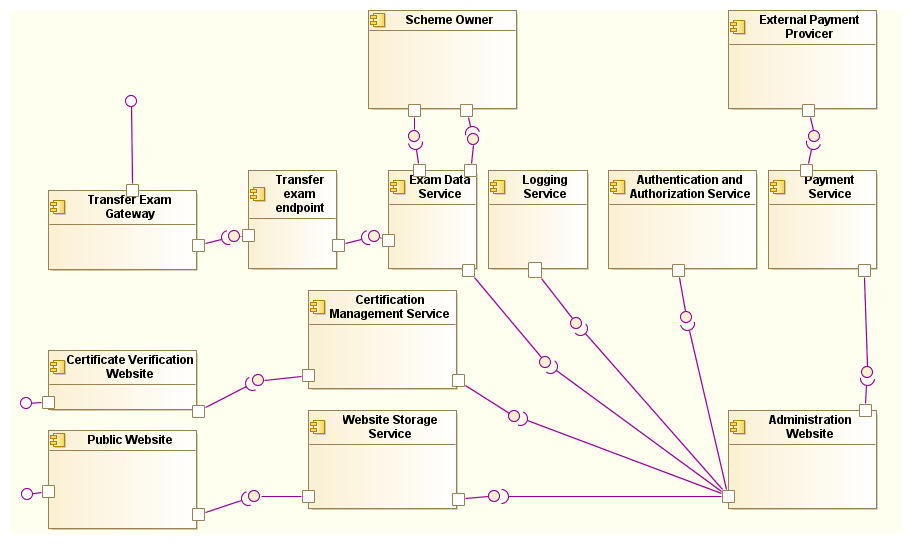
\includegraphics[scale=0.5]{uml/vision2.png}
    \caption{Architektur mit hoher Kohäsion}
\end{figure}

Diese Architektur sollte nun auf die Erfüllung der nicht funktionalen Anforderungen überprüft und gegebenenfalls angepasst werden. Zur Überprüfung der Anforderungen wurden die priorisierten, nicht funktionalen Anforderungen eines Usecases herangezogen. Der Prozess ähnelte damit stark einem szenariobasierten Review wie er in ATAM durchgeführt wird.

Auch dieser Prozess litt jedoch unter dem Problem, dass die nicht funktionalen Anforderungen schwer bewertet werden konnten. Außerdem war es schwer ein Regelwerk/Rezept aus der Architekturerstellung abzuleiten, da durch die Einbeziehung unterschiedlicher AuftraggeberInnen jeweils verschiedene Architekturen entstehen können. Die Einbeziehung von Kohäsion als Aufteilungsgrundlage der Komponenten verursachte zudem ein gefühlt zu großes System, welches in der Umsetzung sehr teuer geworden wäre. Die Kostenersparnis des Systems, welche in der Systemvision definiert wurde, schien damit unzureichend erfüllt zu werden.

\subsection{Von den Daten zu den Komponenten}
Die Auswahl und Bewertung der Komponentenarchitekturen und der starke Fokus auf die nicht funktionalen Anforderungen in den beiden vorherigen Prozessen stellte ein wesentliches Hindernis zur Erstellung eines eindeutigen Regelwerkes dar: Eine vollständige Auflistung aller möglichen Komponentenarchitekturen erschien entweder unmöglich oder unvollständig zu sein; eine Bewertung der nicht funktionalen Attribute schien ohne entsprechende Implementation nur sehr grob überprüfbar zu sein. Der Versuch, ein System mit hoher Kohäsion zu erstellen, endete zudem in sehr teuren Architekturen.

Dies war überraschend, da die populärste Architekturbewertungsmethode, ATAM, stark auf nicht funktionale Anforderungen aufbaute. Als Grund für diese Inkompatibilität wurde der Zeitpunkt der Architekturerstellung vermutet: Durch die fehlende Implementationsphase waren die nicht funktionalen Anforderungen sehr schwer zu bewerten und somit mehr oder weniger nicht überprüfbar. Deshalb wurden sie als Hauptkriterium und Ausgangspunkt für die Architekturerstellung verworfen.

Stattdessen wurde der Fokus auf die Aufspaltung der Daten gelegt. Die Daten wurden anhand Ihrer Vertraulichkeit in unterschiedliche Netze aufgeteilt. Diese Netze wurden dann durch Komponenten miteinander verbunden, die den Zugriff auf die Daten regelten.

\begin{figure}[!htbp]
    \centering
    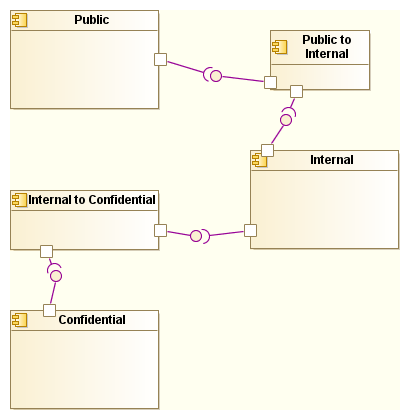
\includegraphics[scale=0.7]{uml/vision3.png}
    \caption{Aufteilung der Komponenten in Datenbereiche}
\end{figure}

Dieser Prozess erlaubte es, eine nachvollziehbare Architektur zu erstellen, jedoch war das Ergebnis zu grob. Außerdem schien eine separate Komponente zur  Übertragung der Prüfungsdaten zu fehlen, welche in der ursprünglichen Systemvision definiert und als notwendig empfunden worden war, um die Rahmenbedingungen der Vertrautheit zu erfüllen \cite[7.3]{ISO_CERT}.

\subsection{Von den Daten und den AkteurInnen zu den Komponenten}
Aufbauend auf dem vorherigen Prozess, welcher die Architektur anhand der Daten erstellte, wurden nun auch AkteurInnen eingebunden und deren Beziehungen zu den Daten ermittelt. Anhand dieser Beziehungen wurden Regeln erstellt, aus denen wiederum die Architektur erstellt wurde.

\begin{figure}[!htbp]
    \centering
    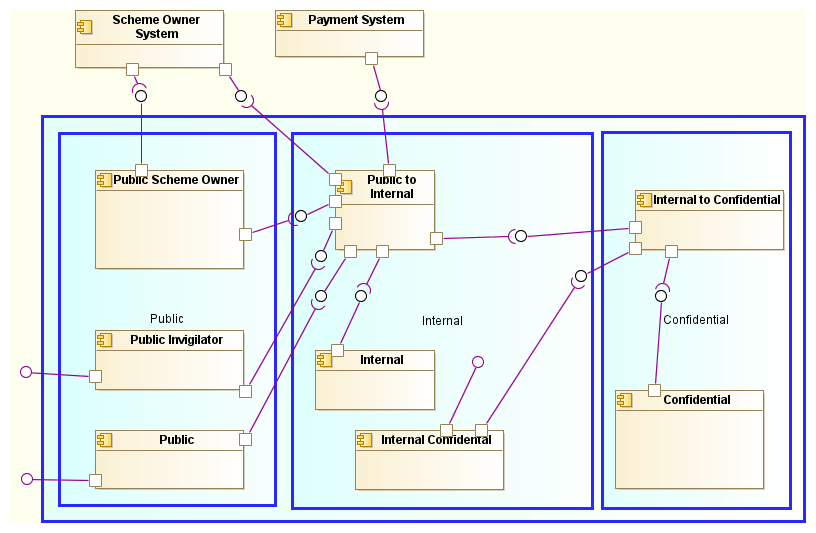
\includegraphics[scale=0.55]{uml/vision4.png}
    \caption{Aufteilung der Komponenten in Datenbereiche und AkteurInnen}
\end{figure}

Dieser Prozess schien nicht nur die Rahmenbedingungen und Sicherheitsbedingungen abzudecken, er war auch durch die erstellten Regeln nachvollziehbar und genau genug, um bereits einen guten Überblick auf die Architektur zu erlangen. Anhand der daraus resultierenden Architektur war es nun auch möglich, nicht funktionale Attribute wie zB. Antwortzeiten besser einschätzen zu können.

\chapter{Prozess Anforderungen}
Da die Software Architektur auf den Anforderungen basiert und viel wichtiger \glqq den gestalterischen Spielraum des Architekten\grqq \cite[S. 103]{softarch} begrenzt, kann davon abgeleitet werden, dass sowohl die Qualität der Architektur als auch die Akzeptanz des Systems wesentlich von den bereits im Vorfeld ermittelten Parametern abhängt. Das bedeutet wiederum, dass für die Klärung der Ausgangsfrage - Wie kommt man von Anforderungen auf eine gute Architektur - auch der Anforderungsprozess eine wichtige Rolle spielt.

Da der Anforderungsprozess ein an sich eigenes, sehr großes Themengebiet dar stellt, wird hier jedoch nur auf die Ausgangsartefakte eingegangen, welche später im Architekturprozess referenziert werden.

\section{Ermittlung der Usecases}
Die Usecases werden zusammen mit dem/der Kundin ermittelt. Daraus wird schlussendlich ein Usecase Diagramm erstellt, welches alle Akteure und Nebensysteme beinhaltet. Dies ist wichtig für das Kontextdiagramm, welches auch im Anforderungsprozess erstellt wird und die Ausgangsbasis für die Architektur dar stellt.

\begin{figure}[!htbp]
    \centering
    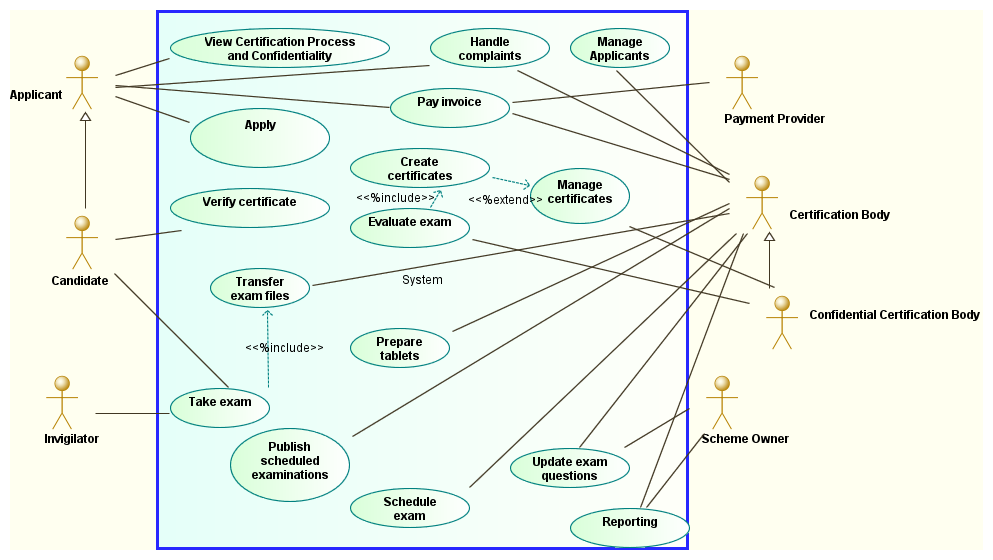
\includegraphics[scale=0.4]{uml/usecase.png}
    \caption{Das mit dem Kunden ermittelte Usecase Diagramm}
\end{figure}

\subsection{Erweiterte Dokumenation der Usecases}
Parallel zur Erstellung des Usecase Diagramms werden zusätzliche Parameter und Beschreibungen für jeden Usecase aufgenommen, welche im eigentlichen Diagramm keine Erwähnung finden.
Dafür wird ein Anforderungstemplate, auch Usecase Beschreibung genannt, verwendet \cite[S. 214]{reqman}, welches aufbauend auf einer Grundversion \cite[Abbildung 8.14, S. 215]{reqman} für jeden Usecase folgende Angaben aufnimmt:

\begin{itemize}
  \item Id: eine eindeutige Bezeichnung, welche dafür verwendet wird, um den Usecase zu referenzieren
  \item Actor: eine Auflistung aller Teilnehmer des Usecases
  \item Description: eine kurze Beschreibung des Usecases
  \item Preconditions: eine Auflistung von Vorbedinungen für den Usecase
  \item Postconditions: eine Auflistung von Nachbedingungen für den Usecase
  \item Normal Course of Events: eine Beschreibung des Standardablaufes
  \item Alternative Courses: Auflistung von Erweiterungen oder zusätzlichen Möglichkeiten
  \item Exceptions: Beschreibung von diversen Ausnahmefälle
  \item Assumptions: Annahmen, unter welcher der Usecase beschrieben wird
  \item Priority: eine Gewichtung, wie wichtig der Usecase ist
  \item Notes: sonstige Anmerkungen
\end{itemize}

Sind die Abläufe komplexer, können Aktivitäts Diagramme verwendet werden, um komplexere Abläufe verständlicher dar zu stellen \cite[S. 215]{reqman}:

\begin{figure}[H]
    \centering
    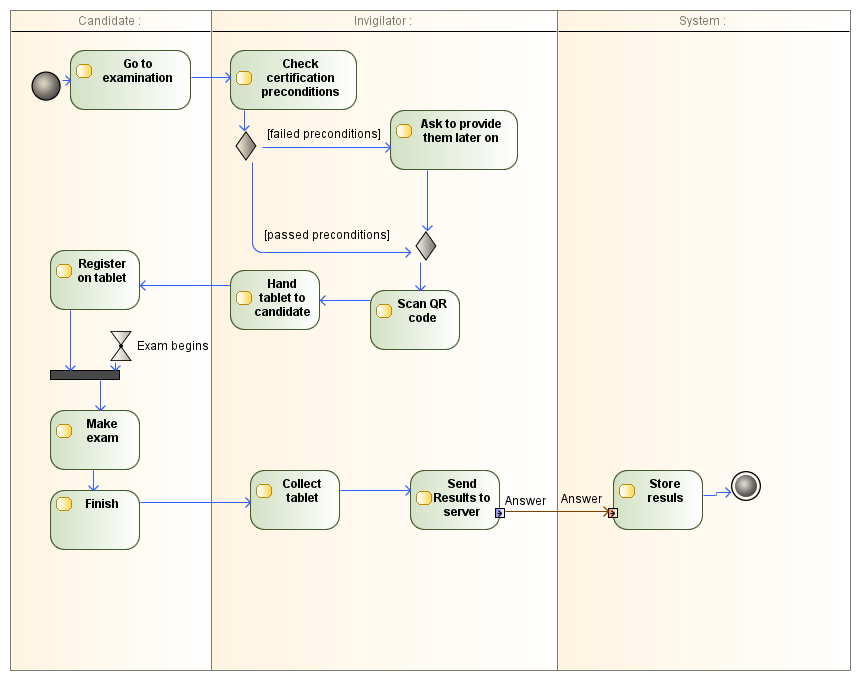
\includegraphics[scale=0.4]{uml/takeexamreq.png}
    \caption{Der Ablauf des Take Exam Usecases im Detail}
\end{figure}

\subsection{Einbeziehen von Architekturreviewparametern}
Um die Einhaltung der Qualitätsparameter zu garantieren, können Architekturreviews durchgeführt werden \cite[S. 20]{review}. Es existiert zwar \glqq keine singuläre, allgemein akzeptierte Metrik um eine Architektur zu beurteilen\grqq \cite[S. 19]{review}, jedoch liefern sie grobe Einschätzungen über die Angemessenheit des Systems \cite[S. 20]{review}. Folgende Architekturreviews wurden dafür ausgewählt:

\begin{itemize}
  \item ATAM: betrachtet Wachstums- und explorative Szenarien um die Architektur zu beurteilen \cite[S. 61]{review}
  \item CBAM: basiert auf ATAM, beachtet jedoch vor allem den Nutzen und die Risiken und Kosten der Architketur, um die Architekturentscheidungen besser abwähgen zu können. Hauptfaktor ist der ROI. \cite[S. 67]{review}
\end{itemize}

Für diese Reviews können bereits früh ein Großteil der benötigten Parameter ermittelt bzw. zumindest grob abgeschätzt werden. Dies ist wichtig, weil nach der 10er Regel der Fehlerkosten früh erkannte Fehler und Probleme weniger Kosten nach sich ziehen als später Erkannte \cite[S. 154]{fehler}.

Deswegen wird das Anforderungstemplate um folgende Parameter erweitert:

\begin{itemize}
  \item Earned Value per month: Wieviel Umsatz der Usecase in einer bestimmten Zeit generiert
  \item Expected Usage: Anzahl der erwarteten Nutzer des Systems pro Zeiteinheit
  \item Growth Scenarios: Anzahl der erwarteten Nutzer des Systems pro Zeiteinheit bei einer höheren Nutzeranzahl
  \item Change Scenarios: mögliche Änderungsszenarien und Erweiterungen
\end{itemize}

\subsection{Einbeziehen von nicht funktionalen Qualitätsattributen}
Nicht funktionale Qualitätsattribute beschreiben die nicht funktionalen Anforderungen an das System. Da Qualität oft schwammig formuliert ist, ist es wichtig, diese Attribute messbar zu machen \cite[S. 9]{effektiv}.

Deswegen werden für jeden Usecase und dessen architekturrelevanten, nicht funktionalen Anforderungen messbare Parameter definiert. Diese Parameter helfen schon im Vorfeld dabei die Architektur zu überprüfen.

Für das Beispielprojekt wurden folgende Parameter definiert, mit welchen das Anforderungstemplate erweitert wurde:

\begin{itemize}
  \item Response Time in Seconds: Wie schnell die Antwort des Systems auf eine Anfrage reagieren muss
\end{itemize}

\section{Rahmenbedingungen}
Zusätzlich zu funktionalen und nicht funktionalen Anforderungen werden auch die Rahmenbedingungen ermittelt, unter welchem das System erstellt werden soll. Diese Anforderungen beinhalten meist den organisatorischen und zeitlichen Ablauf des Projektes und können auch gewisse Technologien vorschreiben, zB. wenn das System in ein bereits bestehendes System integriert werden soll. \cite[S. 9]{review}\cite[S. 110]{softarch}

Die Rahmenbedingungen des Beispielprojektes lassen sich zum Großteil aus dem ISO Standard für Zertifizierungsstellen ermitteln \cite{ISO_CERT} und geben Einsicht in die Vertraulichkeit der Daten und eröffnen weitere Usecases. Sofern möglich werden diese Parameter in das Usecase Diagramm und das Klassen Diagramm der zu verwendeten Daten mit einbezogen. Auf zeitliche und technologische Rahmenbedingungen wurde im Beispielprojekt nicht eingegangen.

\section{Ermittlung der Daten}
Die zu speichernden Daten werden ermittelt und mit Hilfe eines Klassen Diagrammes modelliert. Dies ist nicht nur wichtig und nützlich, weil die Beispielanwendung in diesem Falle eine stark datenzentrierte Anwendung ist \cite[S. 105]{effektiv}, sondern wird später auch einen wesentlichen Beitrag zur Aufteilung des Systems in Komponenten leisten. Im Falle des Beispielprojekts wurden folgende Daten ermittelt und modelliert:

\begin{figure}[H]
    \centering
    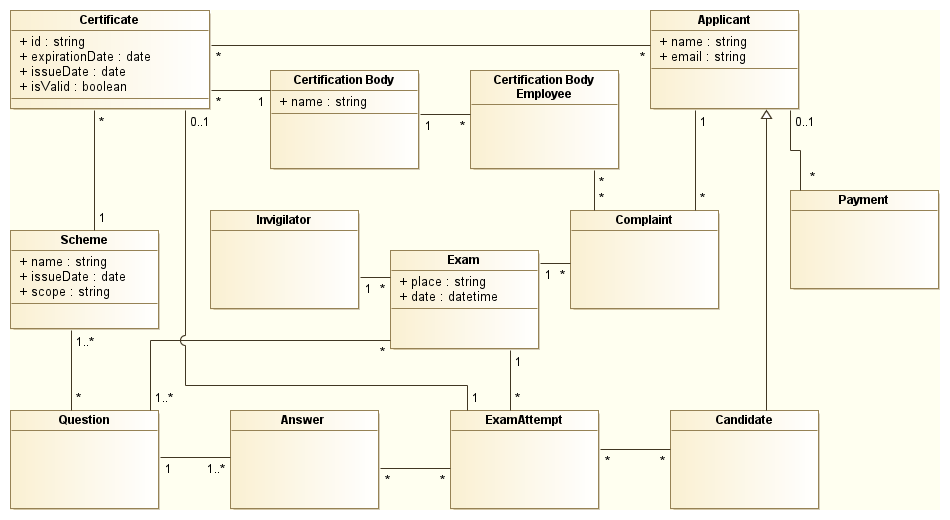
\includegraphics[scale=0.5]{uml/class.png}
    \caption{Das ermittelte Klassendiagramm des Beispielprojektes}
\end{figure}

\section{Ermittlung der Datenvertrautheit}
Nach der Ermittlung der Daten wird auf Basis der Rahmenbedingungen und Sicherheitsstruktur zusammen mit dem/der Kunden/Kundin ermittelt, welche Daten in welche Vertrautheitskategorien fallen. Dazu werden die Daten anhand ihrer gewollten Lesbarkeit in mehrere Untergruppen unterteilt.

Ermittelt wurden in diesem Falle folgende drei Kategorien:

\begin{itemize}
  \item Public: öffentlich zugängliche Daten, welche auf der Webseite zugänglich gemacht werden
  \item Internal: Daten, welche für die inneren Abläufe Betriebs notwendig sind, aber nicht öffentlich zugänglich sein sollen
  \item Confidential: Daten, welche innerhalb des Betriebes verwendet werden, aber eine besondere Geheimhaltungspflicht und Zugriffschbeschränkung benötigen. Dieses Vertrautheitslevel wurde aufgrund der Rahmenbedingung des Vertraulichen Umgangs mit Prüfungsdaten ermittelt \cite[7.3]{ISO_CERT}
\end{itemize}

Um diese Vertrautheitskategorien besser zu visualisieren zu können wird das UML Metamodel mit Hilfe eines Profiles angepasst. Jede Kategorie erhält einen gleich lautetenden Stereotypen \cite[S. 518]{glasklar}:

\begin{figure}[!htbp]
    \centering
    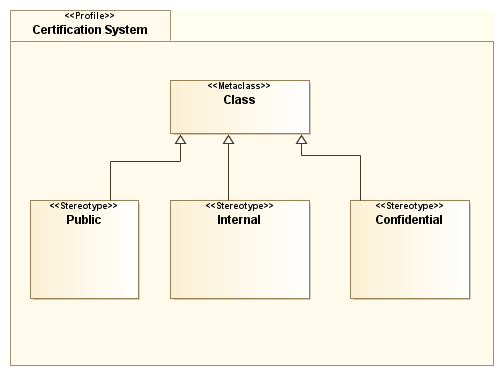
\includegraphics[scale=0.5]{uml/datastereotypes.png}
    \caption{UML wird mit einem Profil um drei Stereotypen erweitert}
\end{figure}

Nach der Erstellung der Stereotypen werden die Daten mit den Vertrautheitskategorien versehen. Sollte es nicht eindeutig sein, welche Klasse in welche Kategorie fällt, müssen die Daten aufgespalten werden und mit einer Assoziation modelliert werden.

\begin{figure}[!htbp]
    \centering
    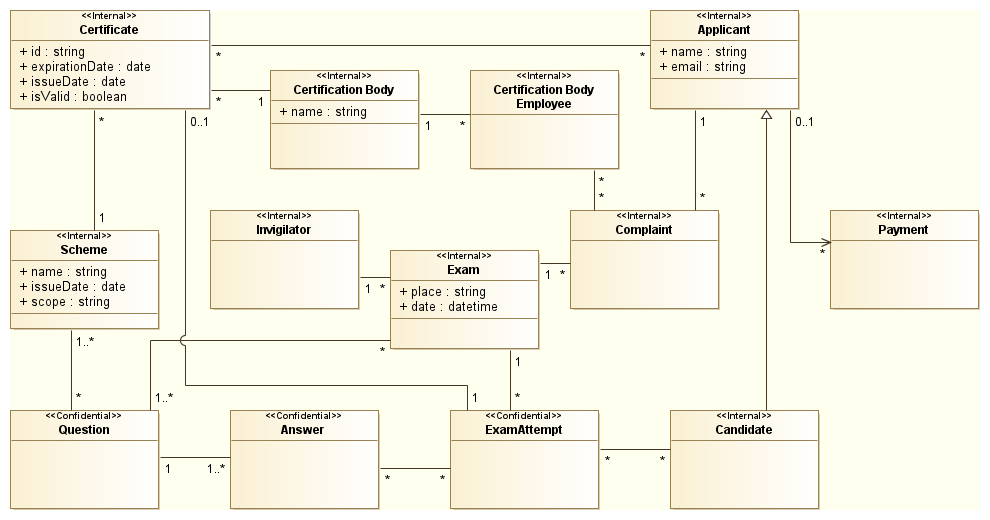
\includegraphics[scale=0.5]{uml/classstereotyped.png}
    \caption{Das Klassendiagramm wird mit Stereotypen der Vertraulichkeit erweitert}
\end{figure}

TODO: datenverlust + angriffsszenarien?

\section{Ermittlung der Akteure und Partnersysteme}
Auf Basis des Usecase Diagrammes können die Akteure und deren Partnersysteme mit Hilfe eines Kontext Diagrammes visualisiert werden

\begin{figure}[!htbp]
    \centering
    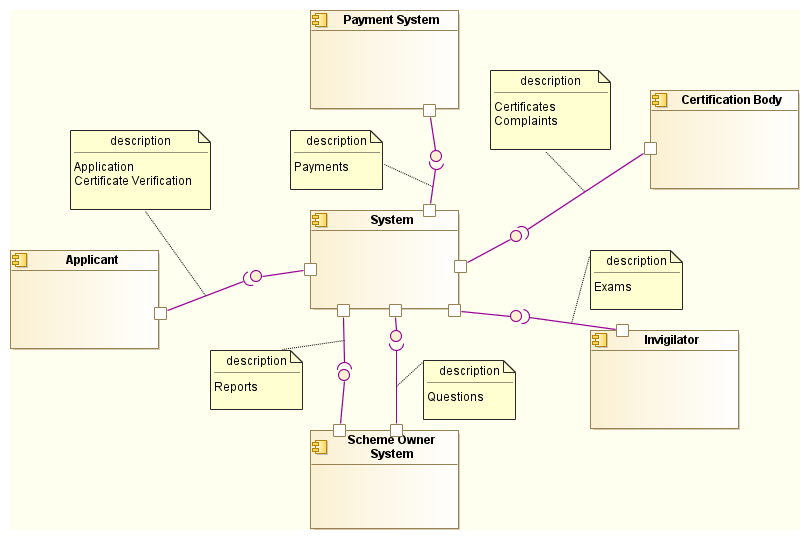
\includegraphics[scale=0.5]{uml/context.png}
    \caption{Das Kontext Diagramm zeigt das System, die Akteure und die Nachbarsysteme}
\end{figure}
\chapter{Erstellung der Architektur}
Aufbauend auf den im Anforderungsprozess ermittelten Attribute, kann nun mit der Architekturplanung begonnen werden. Bereits an dieser Stelle können aufgrund der ermittelten Parameter und Erfahrungswerte eine grundsätzliche Überprüfung der Machbarkeit des Projektes durchgeführt werden. Auch eine Überprüfung, ob der beschriebene Prozess der Architekturplanung für das Projekt eignet kann durchgeführt werden: Der Prozess beschäftigt sich hauptsächlich mit der Aufspaltung und Trennung der Daten und AkteurInnen in mehrere Systeme. Durch außergewöhnlich strenge Laufzeitanforderungen oder entsprechende Rahmenbedinungen kann diese Aufspaltung jedoch zu einer Architektur führen, welche die ursprünglich ermittelten Anforderungen nicht mehr, oder nur schlecht erfüllt.

Die erwähnten Architektursichten werden, soweit möglich, durch UML Diagramme realisert:

\begin{itemize}
  \item Logical View: Klassendiagramm
  \item Process View: Komponentendiagramm, diverse Werte in der Usecasebeschreibung sowie Aktivitäts- und Interface-Klassendiagramm
  \item Development View: Da noch keine Implementation vorhanden ist, können noch keine Bibliotheken und Module beschrieben werden. Hierfür würde sich jedoch das Paketdiagramm anbieten
  \item Physical View: Grobes Komponentendiagramm. Da die Wahl der exakten physischen Komponenten durch die fehlende Implementation nicht früh überprüfbar ist, wurde auf eine Modellierung in der Planungsphase verzichtet
  \item Scenarios: Usecasediagramm
\end{itemize}

\section{Erstellen der minimalen Architektur}
Das Kontextdiagramm, welches im Anforderungsprozess erstellt worden ist, zeigt das System mit allen AkteurInnen und Nachbarsystemen. Aufbauend darauf kann nun die minimale Architektur erstellt werden, welche sich aus dem System und den Nachbarsystemen ableitet.

\begin{figure}[H]
    \centering
    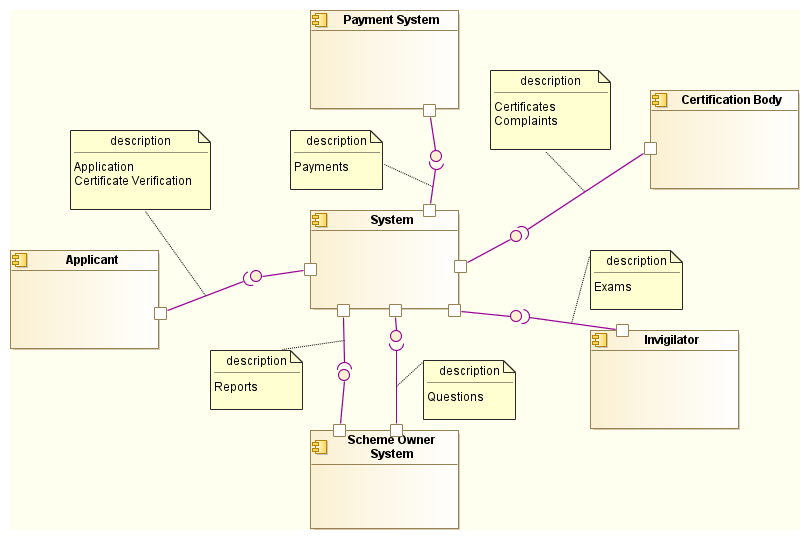
\includegraphics[scale=0.5]{uml/context.png}
    \caption{Das Kontextdiagramm liefert die Ausgangsbasis für die Architektur}
\end{figure}

Zuerst werden alle Datenflussnotizen entfernt. Danach werden alle Komponenten entfernt, welche kein eigenes System darstellen. In diesem Falle werden folgende Komponenten entfernt:

\begin{itemize}
  \item Applicant
  \item Certification Body
  \item Invigilator
\end{itemize}

Dies führt zu folgender Minimalarchitektur:

\begin{figure}[H]
    \centering
    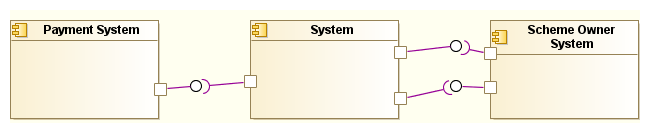
\includegraphics[scale=0.7]{uml/minimalarch.png}
    \caption{Minimale Architektur}
\end{figure}

Für die Nachbarsysteme selbst wird keine Architektur erstellt, jedoch beeinflussen sie die Schnittstellen des Systems und sind deswegen wichtig für den weiteren Prozess. Sie werden in die Architektur einbezogen.

\section{Erstellen der Datenminimalarchitektur}
Auf Basis der im Anforderungsprozess ermittelten Zonen wird das System der vorher erstellte Minimalarchitektur in ebenso viele Teilsysteme unterteilt. Die Aktivitätsdiagramme werden an die neue Architektur angepasst: Für jedes Untersystem wird in den Diagrammen eine eigene Swimlane erstellt. Die involvierten AkteurInnen sind, falls möglich, als eigene Swimlane modelliert, spielen in dieser Phase aber noch keine wichtige Rolle zur Gliederung des Systems.

\begin{figure}[H]
    \centering
    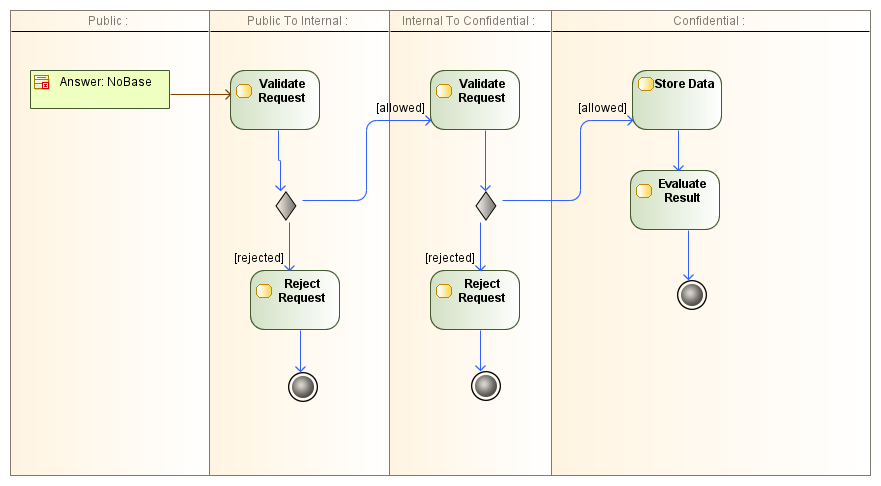
\includegraphics[scale=0.5]{uml/takeexamactivity1.png}
    \caption{Die Antworten werden nach der Prüfung an den Certification Body übermittelt. Der Request wird dann durch zwei Gateways zum finalen System geleitet.}
\end{figure}

Wechselt der Kontrollfluss eine Swimlane eines Systems, heißt dies, dass eine Verbindung zwischen den beiden sonst abgeschotteten Systemen benötigt wird. Dieses Verbindung wird als eigene Komponente modelliert und wird als Gateway bezeichnet. Die Aufgabe dieses Gateways ist es, folgende Attribute der Anfrage zu überprüfen und die Anfrage gegebenenfalls zu verwerfen oder weiterzuleiten:

\begin{itemize}
  \item Von welchem System kommt die Anfrage?
  \item Welches System ist das Ziel der Anfrage?
  \item Welche Schnittstelle dieses Systems ist das Ziel der Anfrage?
  \item Gibt es eine Regel die diese Anfrage explizit erlaubt?
\end{itemize}

Der Gateway fungiert damit als eine Art Application Firewall.

Der Gateway ist jedoch nicht der einzige Punkt an welchem der Zugriff auf Schnittstellen autorisiert wird. Er ist viel mehr ein zusätzlicher Layer, der den Zugriff auf die Schnittstellen absichert. Überwindet ein/eine AngreiferIn durch einen Fehler im Gateway diese Kontrolle, hat er/sie zwar Zugriff zum Internal System, kann aber trotzdem nocht nicht auf die Daten zugreifen, da diese eine zusätzliche Authentifizierung benötigen. \cite{sec}[S. 350]

Die anfangs beschriebenen Nachbarsysteme werden nach ihren Anforderungen, welche aus den Aktivitätsdiagrammen ablesbar sind, an das System in ihrer Zone angeschlossen. Ist das Ausgangssystem ein System, welches nicht vom/von der AuftraggeberIn kontrolliert wird, und greift das Ausgangssystem von einer Zone mit einer niedrigeren Vertrautheitsebene auf ein Zielsystem mit einer höheren Vertrautheitsebene zu, muss dies jedoch über ein zusätzliches System erfolgen. Dies ermöglicht es, den Gateway komplett von unkontrollierten Systemen abzukapseln und dessen Angriffsfläche zu verringern. Dies ist besonders wichtig, weil der Gateway bei Angriffen einen Single Point of Failure darstellt.

Das Beispielprojekt bezieht Zahlungsdaten direkt von einem Payment System und die Prüfungsfragen werden direkt an das Scheme Owner System gesandt. Beides Ausgangssysteme dieser Anfragen stammen aus einem System mit einer höheren Vertrautheitsebene als dem Zielsystem und benötigen deswegen kein eigenes Zwischensystem, sprich können direkt über den Gateway zum Ziel geführt werden. Dem entgegen gesetzt ist die Übermittlung der Prüfungsfragen des Scheme Owner Systems: Das Ausgangssystem greift hier von einem nicht kontrollierten System und einer niedrigeren Vertrautheitsebene auf eine Zielsystem in einer höheren Vertrautheitsebene zu, was eine zusätzliche Komponente nötig macht.

\begin{figure}[H]
    \centering
    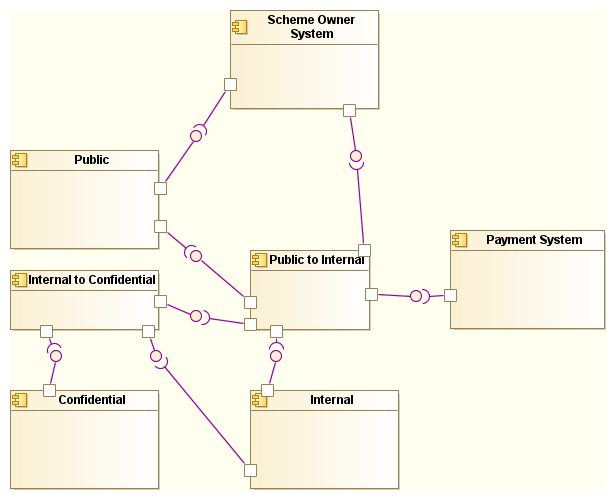
\includegraphics[scale=0.7]{uml/dataarch.png}
    \caption{Aufteilung der Komponenten in Datenbereiche}
\end{figure}

Eine weitere wichtige Regel ist, dass keine Gateways unterschiedlicher Vertrautheitsebenen übersprungen werden dürfen. Zeigt ein Aktivitätsdiagramm zB. einen Zugriff von Ebene 1 auf Ebene 3 muss dieser Zugriff sowohl durch den Gateway der Ebene 2, als auch durch den Gateway der Ebene 3 geleitet werden. Dies verhindert, dass besonders schützenswerte Systeme direkt an Systeme mit einer weitaus niedrigeren Vertrautheitsebene angeschlossen werden und so dessen Gateway zum Single Point of Failure wird. Dies gilt in beide Richtungen.

Da bei der Erstellung des Systems nun alle Schnittstellen und Systeme bekannt sind, können diese Regeln fest im Gateway verankert werden. Weil diese Gateways unabhängig voneinander agieren, können sie durch das Hinzufügen eines Load Balancers beliebig vervielfacht werden, was sowohl die Ausfallsicherheit als auch die Skalierbarkeit erhöht. Das ist wichtig, weil sie als einzige Verbindung zwischen den Systemen zu einer Art Flaschenhals werden.

\section{Einbinden der AkteurInnen}
Nachdem die Datenminimalarchitektur steht, können nun die AkteurInnen des Systems in die Aufgliederung des Systems mit einbezogen werden. Hierfür müssen nun die Objektflüsse und die AkteurInnen des Systems für jeden Usecase betrachtet werden, welche aus den vorher bereits erstellten Aktivitäts- und Kontextdiagramm ersichtlich sind.

Zuerst wird das erste Untersystem, in diesem Falle das Public System, betrachtet. Alle Objektflüsse durch das System und die AkteurInnen, welche mit ihren Swimlanes angrenzen, sind in die Aktivitäten des Systems involviert. Jede Involvierung eines/einer Akteurs/Akteurin in ein System erfordert einen Zugang zu diesem System.

Jeder dieser AkteurInnen muss mit den minimal möglichen Rechten für dieses System ausgestattet werden, um seine Aufgaben zu erfüllen. Dies vermeidet nicht nur Fehler sondern reduziert auch den Schaden, welcher ein potentieller Angriff dieses Akteurs/dieser Akteurin anrichten kann \cite[1. A]{leastpriv}.

Da ein System komplex ist \cite[S. 7]{softarch}, und diese Sicherheitsattribute nach Änderungen am System immer wieder überprüft werden müssen, stellt jeder zusätzliche Zugriff eines/einer Akteurs/Akteurin nicht nur ein Sicherheitsrisiko dar, sondern erhöht auch den Test- und damit den Wartungsaufwand. Idealerweise wird daher jedem/jeder AkteurIn ein eigenes, für sich abgekapseltes System zur Verfügung gestellt, was jedoch meist aufgrund Kosten der zusätzlichen Systeme keine Option dar stellt.

Um zu ermitteln, welche Systeme eine eigene Komponente benötigen, wird nun entweder anhand einer Tabelle oder zusammen mit dem/der KundIn pro Usecase und deren Komponenten ermittelt, ob der Schaden eines unerlaubten Zugriffs der Daten den eines Systems überschreitet. Die Schadens- und Systemkosten müssen zuerst von dem/der KundIn und dem/der ArchitektIn geschätzt werden.

Im Falle des Beispielprojektes wurde auf Basis des folgenden stark vereinfachten Aktivitätsdiagramms in Abbildung \ref{fig:actorarch} ermittelt, dass die möglichen Schadenskosten im Falle, dass der/die AnwärterIn (Applicant) Zugriff auf die Prüfungsantworten (Answer) bekommt, die eines eigenen Systems überschreiten. Das gleiche Problem trifft auch auf den Scheme Owner zu: die Schadenskosten im Falle einer Manipulation oder eines lesenden Zugriffes des/der AnwärterIn (Applicant) auf die Fragen überschreitet auch hier die Kosten eines eigenen Systems. Deswegen werden zwei zusätzliche Systeme erstellt und aus dem Public System ausgegliedert.

Für den Fall, dass bei der Aufspaltung zu viele Systeme entstanden sind, werden nun in einem weiteren Schritt diverse Kombinationen von Teilsystemen betrachtet und versucht zusammen zu legen, solange deren Schadenskosten nicht die Systemkosten überschreiten. Gibt es mehrere mögliche Kombinationen, entscheidet das in den Anforderungen aufgenommene Related Usecases Feld und danach die Überschneidung der Datentypen über die genaue Aufteilung. Ändert sich ein Usecase, so sind meist auch andere Usecases von dieser Änderung betroffen. Je weniger Komponenten nach einer Änderung betrachtet werden müssen, desto niedriger sind die Wartungskosten.

Beim Beispielprojekt zeigt sich, dass es keine erlaubte Kombination gibt, da die Schadenskosten jeweils weit über den Kosten eines eigenen Systemes liegen. Es bleibt somit bei den ermittelten zwei Zusatzsystemen.

\begin{figure}[H]
    \centering
    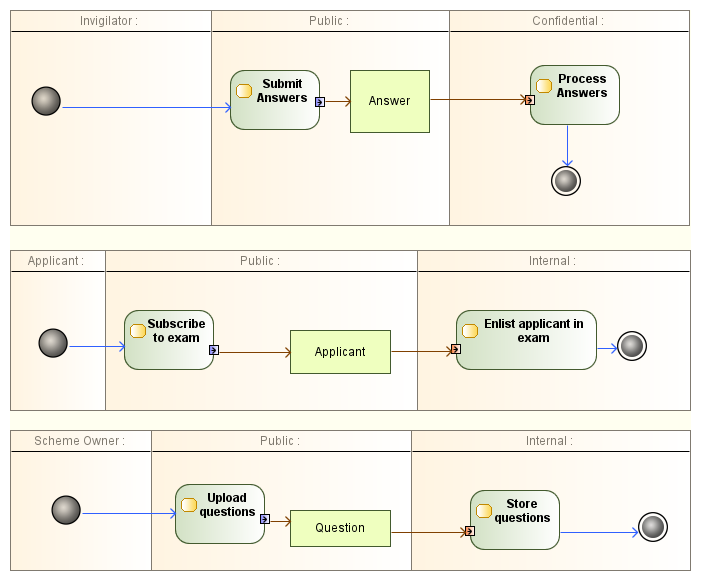
\includegraphics[scale=0.6]{uml/actorarch.png}
    \caption{Vereinfachte Gegenüberstellung von Aktivitätsdiagramme für das Public System}
    \label{fig:actorarch}
\end{figure}

Diese Analyse wird für alle verbleibenden Systeme durchgeführt, bis alle Systeme aufgespalten sind.

Im Falle des Beispielprojektes führt dies schlussendlich zu folgender Systemaufspaltung:

\begin{figure}[H]
    \centering
    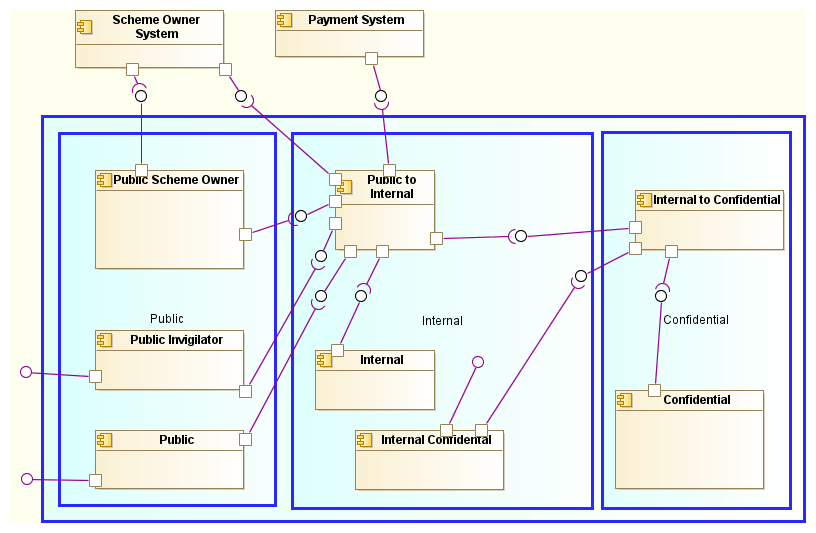
\includegraphics[scale=0.6]{uml/vision4.png}
    \caption{Architektur nach der Aufspaltung }
\end{figure}

\section{Analyse der nicht funktionalen Attribute}
Ist die erste Version der Architektur erstellt, kann nun mit der grundsätzlichen Überprüfung der im Anforderungsprozess ermittelten Parameter begonnen werden, welche bereits wichtige Informationen und Rückschlüsse auf den jetzigen Status der Architektur geben. Basierend auf den Usecases, den ermittelten Komponenten der Architektur und den Aktivitätsdiagrammen wird eine Tabelle erstellt, welche Auskünft darüber gibt, welche Komponenten für jeden Usecase benötigt werden. Diese Tabelle dient als Basis für weitere Analysen.

Um herauszufinden, welche Komponenten für einen Usecase benötigt werden, können die Swimlanes der Aktivitätsdiagramme herangezogen werden. Da für AkteurInnen keine Komponente gelistet werden, werden deren Swimlanes ignoriert. Ein Beispiel hierfür ist das Aktivitätsdiagramm des Handle Complaint Usecases in Abbildung \ref{fig:handlecomplaintreview}.

\begin{figure}[H]
    \centering
    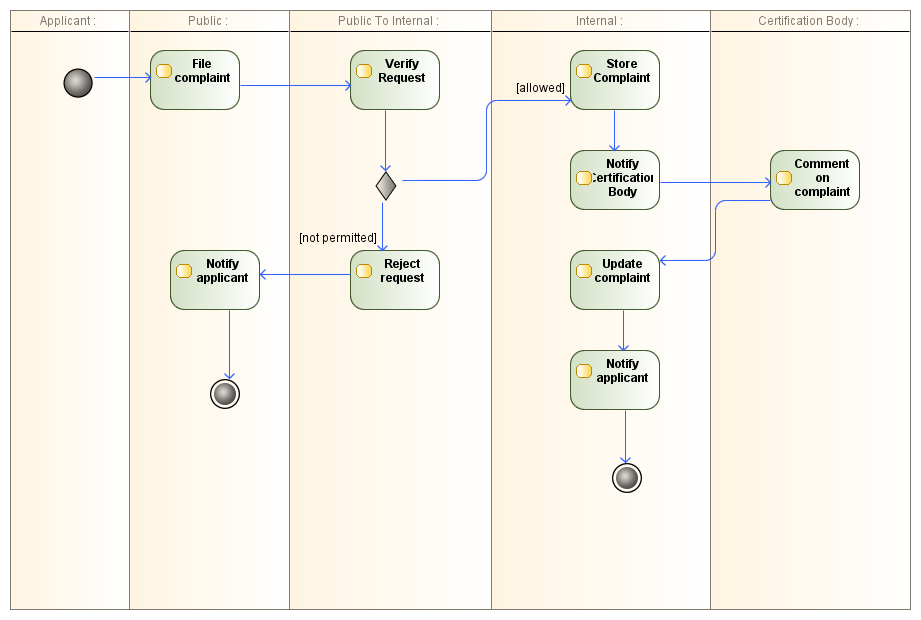
\includegraphics[scale=0.5]{uml/handlecomplaintsactivityreview.png}
    \caption{Vereinfachtes Aktivitätsdiagramm des Handle Complaints Usecases mit der id complaints}
    \label{fig:handlecomplaintreview}
\end{figure}

Werden die beiden AkteurInnen entfernt, bleiben für diesen Usecase folgende Komponenten übrig:

\begin{itemize}
  \item Public
  \item Public To Internal
  \item Internal
\end{itemize}

Diese werden nun in eine Tabelle überführt, wobei für jede verwendete Komponente eines Usecases mit einem x markiert wird:

\hfill \break

\begin{tabular}{ | r | c | }
    \hline
    Komponenten & complaints \\
    \hline
    Public & x \\
    \hline
    Public Invigilator & \\
    \hline
    Public Scheme Owner & \\
    \hline
    Public To Internal & x \\
    \hline
    Internal & x \\
    \hline
    Internal Confidential & \\
    \hline
    Internal To Confidential & \\
    \hline
    Confidential & \\
    \hline
    Scheme Owner System & \\
    \hline
    Payment System & \\
    \hline
\end{tabular}

\hfill \break

Dies wird für alle Usecases durchgeführt und führt im Falle des Beispielprojektes zu folgender Matrix:

\begin{figure}[H]
    \centering
    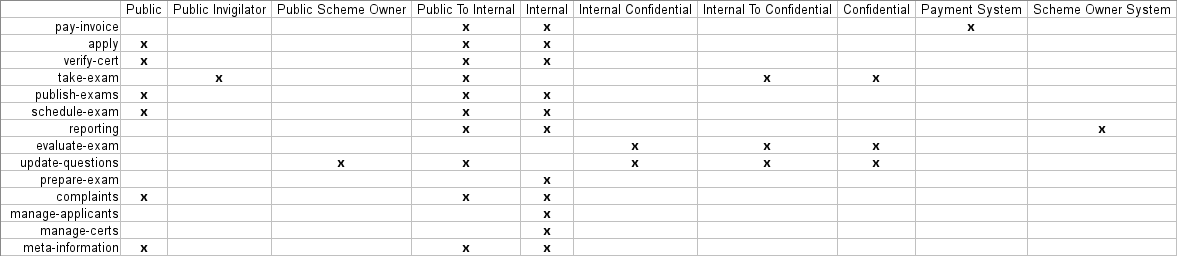
\includegraphics[scale=0.4]{img/matrix.png}
    \caption{Matrix der Komponenten und Usecases des Beispielprojektes}
    \label{fig:matrix}
\end{figure}




\subsection{Reliability}
Anhand der in ermittelten Usecase und Komponenten Matrix kann nun sowohl eine Überprüfung der der Ausfallskosten als auch eine Single Point of Failure Analyse durchgeführt werden.

\subsubsection{Single Point of Failure Analyse}

Ein Single Point of Failure beschreibt eine Komponente, die so kritisch für das System ist, dass ihr Ausfall den kompletten Ausfall des Systems nach sich zieht \cite[S. 3]{single}. Ein Single Point of Failure der Architektur kann daran erkannt werden, dass eine Komponente in allen Usecases vorkommt. Im Bezug auf die soeben ermittelte Matrix wird dies durch eine durchgehende Reihe von mit x markierten Zellen in der Komponentenspalte ersichtlich.

Enthält eine Architektur einen Single Point of Failure, muss diese Komponente entweder redundant ausgelegt sein, oder es muss eine Aufspaltung anhand einer Fehlerkostenanalyse durchgeführt werden.

Im Falle der Matrix in Abbildung \ref{fig:matrix} ist keine durchgehende Reihe an markierten Zellen erkennbar und somit existiert kein Single of Failure. Es lässt sich einzig und allein ablesen, dass die Public To Internal und Internal Komponente eine Abweichung vom Single Point of Failure um vier respektive drei besitzen. Dies lässt erahnen, dass bei der Implementation und Wartung dieser Systeme besondere Sorgfalt von Nöten ist.

\subsubsection{Ausfallkosten Analyse}
Zusätzlich zu einer Single Point of Failure Analyse gibt eine Ausfallkosten Analyse auf Basis des in den Anforderungen ermittelten Monatsumsatzes Auskunft darüber, welche Komponenten jeweils wieviel Umsatz generieren. Für diese Überlegung können auch die Wachstumsszenarien einbezogen werden, falls sich der Umsatz durch eine Steigerung der BenutzerInnen steigert oder senkt.

Das Ergebnis dieser Analyse ist die notwendige Redundanz der einzelnen Komponenten, welche bei der Implementation des Systems erreicht werden muss.

Die nachfolgenden Berechnungen verteilen den Schaden aus Gründen der Einfachheit gleichmäßig auf alle Zeiteinheiten. Es kann sein, dass eine Organisation so strukturiert ist, dass ein eintägiger Ausfall keine Umsatzeinbußen nach sich zieht. In diesem Falle ist die Beispielrechung ungenau. Um diese Möglichkeit einzubeziehen, müssen detailiertere Umsatzkosten im Anforderungsprozess ermittelt werden was jedoch aus Gründen des Umfangs und der Einfachheit vermieden wird. Das Beispiel soll lediglich als ein anschauliches Beispiel zur Ermitllung des Umsatzrückganges dienen.

Um den monatlichen Umsatz der Komponenten zu ermitteln, wird das x in den markierten Feldern mit dem Monatsumsatz des Usecases ersetzt. Leere Felder werden mit 0 aufgefüllt. Schlussendlich werden alle Werte einer Komponente addiert, um den Gesamtumsatz zu ermitteln.

Als Beispiel dient hier die Internal Komponente (Die Werte sind beispielhaft gewählt):

\hfill \break

\begin{tabular}{ | r | c | }
    \hline
    Usecases & Internal \\
    \hline
    pay-invoice & 3000 \euro \\
    \hline
    apply & 1500 \euro \\
    \hline
    verify-cert & 1500 \euro \\
    \hline
    take-exam & 0 \euro \\
    \hline
    publish-exams & 1500 \euro \\
    \hline
    schedule-exam & 1500 \euro \\
    \hline
    reporting & 1500 \euro \\
    \hline
    evaluate-exam & 0 \euro \\
    \hline
    update-questions & 0 \euro \\
    \hline
    prepare-exam & 80000 \euro \\
    \hline
    complaints & 1500 \euro \\
    \hline
    manage-applicants & 1500 \euro \\
    \hline
    manage-certs & 1500 \euro \\
    \hline
    meta-information & 1500 \euro \\
    \hline
    Total Sum & 96500 \euro \\
    \hline
\end{tabular}

\hfill \break

Fällt diese Komponente für einen kompletten Monat aus, verursacht sie einen Umsatzrückgang von 95500 \euro. Wenn eine Komponente eine Ausfallwahrscheinlichkeit von 99\% besitzt, dann belaufen sich die durchschnittlichen Ausfallkosten auf 965 \euro. Wird aus Redundanzgründen eine weitere Komponente hinzugefügt und damit die Ausfallwahrscheinlichkeit auf zB. 99.9\% gesteigert, belaufen sich die Schadenskosten nur noch auf 96.5 \euro. Kostet diese zusätzliche Komponente weniger als die Differenz der Kosten, sprich weniger als 868.5 \euro, rentiert sich die Anschaffung einer zweiten Komponente.

\subsection{Usability}
Da die Artefakte des Planungsprozesses keine Oberflächen beschreiben ist eine Auswertung der des nicht funktionalen Parameters Usability nicht möglich. Außerdem ist sie nicht im Fokus der Architekturerstellung und die Überprüfung der Usability kann somit übersprungen werden.

\subsection{Efficiency}
Es ist schwierig, die Effizienz und Performance der Architektur in diesem Stadium zu messen, da noch keine Implementation vorhanden ist und somit weder die Performance noch der Speicherverbrauch des Systems getestet werden können. In diesem Stadium lassen sich lediglich Werte schätzen. Eine Möglichkeit um zB. die Antwortzeiten zu schätzen, ist es, die Anzahl der Swimlanewechsel eines Usecases zu addieren und das Ergebnis mit einer konstanten Zeit, welche auf Erfahrungswerten basiert, zu multiplizieren. Dieser Wert kann dann mit den im Anforderungsprozess ermittelten Antwortzeiten verglichen werden, um zu überprüfen, ob das System diese Anforderungen erfüllt.

Ausgegangen wird hier von den bestehenden Aktivitätsdiagrammen. Je nachdem, für welchen Abschnitt die in den Anforderungen ermittelten Werte gelten, kann nicht der komplette Ablauf des Aktivitätsdiagrammes für die Berechnung der Zeit verwendet werden.

Überschreitet der berechnete Wert den in den Anforderungen ermittelten Wert, muss dessen Kategorie hinzugezogen werden. Ist der Wert nur eine Empfehlung, so wird der Usecase in der Implementationsphase mit einem besonderen Augenmerk auf Geschwindigkeit umgesetzt. Ist der Wert jedoch verbindlich, so muss mit dem/der KundIn Rücksprache gehalten werden \cite[S. 70]{effektiv}: Entweder ist die Anforderung unter diesen Parametern nicht umsetzbar, oder es muss ein Kompromiss zu lasten von anderen Anforderungen eingegangen werden.

Ein Beispiel für die Berechnung der Antwortzeiten wird aus dem Aktivitätsdiagramm des Beispielprojektes für die Anmeldung eines Kandidaten erläutert (Abbildung \ref{fig:applycomplicated}):

\begin{figure}[H]
    \centering
    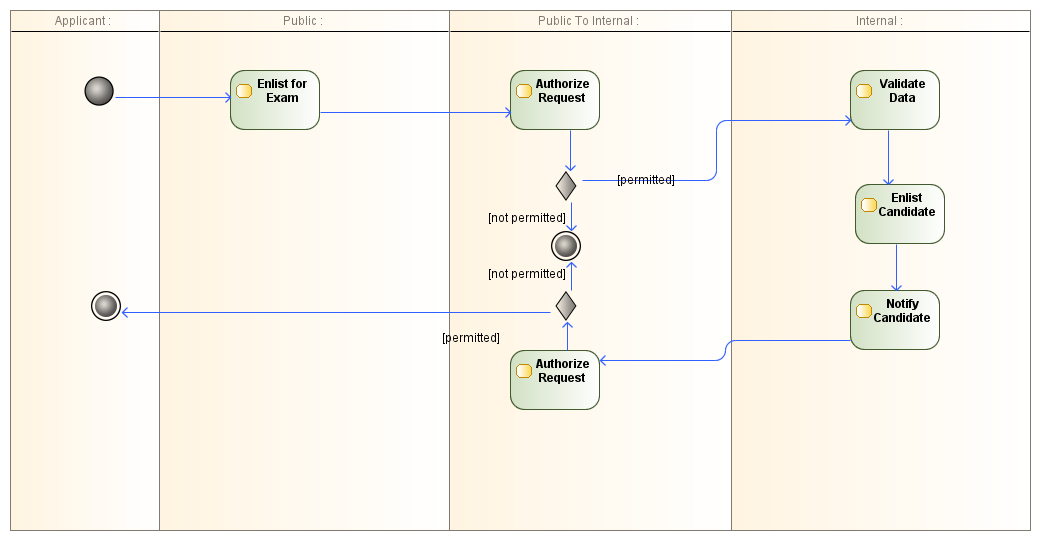
\includegraphics[scale=0.4]{uml/applycomplicated.png}
    \caption{Der Kandidat meldet sich für eine Prüfung an}
    \label{fig:applycomplicated}
\end{figure}

Hier werden, ausgegangen vom Startpunkt sechs Swimlanewechsel gezählt. Diese werden nun mit der Konstante 100 Milisekunden multipliziert, was eine geschätzte Durchlaufzeit von 600 Milisekunden ergibt. Dies liegt unter den erforderlichen 1000 Milisekunden der aufgenommenen nicht funktionalen Anforderung der Antwortzeit.

\subsection{Maintainability}
Maintainability dreht sich um Wart- und Änderbarkeit eines Projektes. Die Änderbarkeit der Architektur hängt wesentlich von der Kopplung und Kohäsion der Komponenten ab. Die Wartbarkeit kann unter anderem an den Wartungskosten abgelesen werden.

\subsubsection{Kopplung und Kohäsion}
Die Änder- und Wartbarkeit ist wesentlich von den Beziehungen der Komponenten und Usecases abhängig. Wird eine Komponenten geändert, so müssen zusätzlich zu dieser Änderung auch eine erneute Validierung der bereits bestehenden Funktionen durchgeführt werden, um Fehler, welche aus den Änderungen entstanden sind, zu finden. Dieses Problem wird mit dem Begriff Ripple Effect beschrieben. \cite[S. 3]{ripple}

Wird ein Usecase geändert, so müssen eine oder mehrere Komponenten des Usecases angepasst werden. Wird eine Komponenten geändert, so kann dies auch andere Usecases beeinflussen, welche die gleiche Komponente verwenden. Wie sehr eine Komponente andere Usecases beeinflusst, kann aus den Komponenten Spalten der Matrix abgelesen werden, in dem die Anzahl der mit x markierten Spalten durch die Anzahl der Gesamtusecases dividiert wird. Der daraus resultierende Wert liegt in den Grenzen von 0 (bester Wert) und 1 (schlechtester Wert) und gibt die Kopplung der Komponente an. \cite[S. 164]{effektiv}

Die Kohäsion beschreibt die inhaltliche Zusammengehörigkeit der Komponenten \cite[S. 164]{effektiv}. Sie kann aus den der Usecase-, Aktivitäts und Klassendiagrammen ermittelt werden. Das Klassendiagramm beschreibt die Zusammengehörigkeit der Daten, das Aktivitätsdiagramm eines Usecases und dessen Objektflüsse die gemeinsam verwendeten Daten. Die Usecases können nun anhand der verwendeten Daten in mehrere unabhängige Gruppen unterteilt werden, die orthogonal zueinander sind. Je mehr unabhängige Gruppen auf eine Komponente zugreifen, desto schlechter ist deren Kohäsion.

Zusätzlich können nun die in den Anforderungen ermittelten Änderungsszenarien mit einbezogen werden. Hat eine Komponente einen hohen Kopplungswert und/oder eine niedrigen Kohäsion, und ist sie Teil eines Usecases, welcher viele Änderungsszenarien beinhaltet, kann dies als Grund zu einer weiteren Aufspaltung der Komponente genommen werden. Gateways sind von Aufspaltungen ausgenommen, da sie als Firewall agieren und so simpel wie möglich konfiguriert werden müssen, um Konfigurationsfehler zu vermeiden.

Wird eine Aufspaltung durchgeführt, so werden sie anhand der in Kohäsionsanalyse ermittelten Gruppen aufgeteilt. Die Priorität der Gruppen wiederum ergibt sich aus den ermittelten Änderungsszenarien, danach werden die in der Ausfallskostenanalyse ermittelten Kosten einer Komponente herangezogen. Diese Ordnung ergibt sich aus der Erkenntnis, dass die Wartung der Software oft mehr als 50\% der Gesamtsystemkosten des Systems ausmacht \cite[S. 71-84]{maincost}.

Die Änderungsszenarien und die Kopplungswerte stellen schlecht bewertbare Werte dar. Zudem kann eine feste Aufteilung anhand der unabhängigen Gruppen der Kohäsion zu einem System führen, in welchem jeder kleine und unabhängige Usecase ein eigenes System bekommt, was wiederum zu einer zu starken Fragmentierung führen kann. Deshalb kann hier keine starre Regel festgelegt werden, wann ein System aufgespalten werden muss und wann nicht. Diese Entscheidung muss vom/von dem/der ArchitektIn selbst getroffen werden.

Wird das Beispielprojekt auf Kohäsion und Kopplung analysiert, fallen vor allem die Internal und Public To Internal Komponente auf, da sie in mehr als der Hälfte aller Usecases eingesetzt werden (Kopplungswert größer als 0.5). Weil die Public To Internal Komponente ein Gateway ist, kann sie ignoriert werden. Damit verbleibt die Internal Komponente. Wird die Kohäsion der Internal Komponente betrachtet, sticht hervor, dass in dieser Komponente mehrere komplett unabhängige Daten verwendet werden: Zahlungen, Zertifikate, Anmeldungen und Beschwerden sind jeweils eigene, logische Gruppen.

Aufgrund der Größe des Systems und der wenigen Änderungsszenarien wurde gegen eine weitere Aufspaltung entschieden, jedoch wurde fest gestellt, dass die Internal Komponente bei der Erstellung der Testfälle eine höhere Testabdeckungen benötigt.

\subsubsection{Wartungskosten}
Die Wartungskosten ergeben sich sowohl aus dem Personal, welches für die Wartung der Komponenten angestellt werden muss, als auch aus den Strom- und Reparaturkosten der eingesetzten Systeme. Weil die genauen Komponenten noch nicht implementiert wurden, kann an diesem Moment nur eine Schätzung der Kosten durchgeführt werden.

Eine einfache Möglichkeit zur Schätzung der Kosten kann durch die Wahl einer Konstanten pro System durchgeführt werden. Im Falle des Beispielprojektes wird pro System mit folgenden monatlichen Kosten gerechnet:

\begin{itemize}
  \item Stromkosten: 10 \euro
  \item Reparaturkosten: 20 \euro
  \item Personalkosten: 100 \euro
\end{itemize}

Die aufsummierten Kosten ergeben Wartungskosten von 130 \euro \ pro Monat. Wird dies mit der Anzahl der Systeme multiplizert ergibt sich ein Gesamtwartungskostenaufwand von 8 * 130 \euro, sprich 1040 \euro \ pro Monat.

\subsection{Portability}
Die Portabilität der Platform kann im Moment noch nicht überprüft werden, da noch keine Festlegung des Projektes auf eine Plattform und/oder Technologie existiert. Dies kann erst zu Beginn der Implementationsphase entschieden werden und wird unter anderem von den in der Anforderungsphase ermittelten Rahmenbedingungen beeinflusst.


\section{Modellierung der Komponentenschnittstellen}
Sind alle Analysen der Architektur abgeschlossen, kann nun anhand der Usecase-, Klassen und Aktivitätsdiagramme damit begonnen werden, die Schnittstellen der Komponenten zu definieren. Die Schnittstellen werden als Interfaces in einem Klassendiagramm modelliert und schlussendlich in das Komponentendiagramm integriert.

Um die unterschiedlichen erlaubten Zugriffe zu modellieren, kann Vererbung genutzt werden: gemeinsame Schnittstellen werden in eine Basisklasse ausgelagert. Obwohl der Gateway bereits einen Großteil der Zugriffe regelt, sind wie in Kapitel 7.2 beschrieben zusätzliche Überprüfungen der Zugriffe von Nöten. Eine Visualisierung dieser verschiedenen Zugriffsrechte ist somit von Vorteil.

Ein Beispiel dafür ist die Beschwerdenschnittstelle des Beispielprojektes, welches sowohl eine Interne als auch eine Public Schnittstelle anbietet. Beide Schnittstellen haben gemeinsame Operationen, welche mit Vererbung modelliert wurden.

\begin{figure}[H]
    \centering
    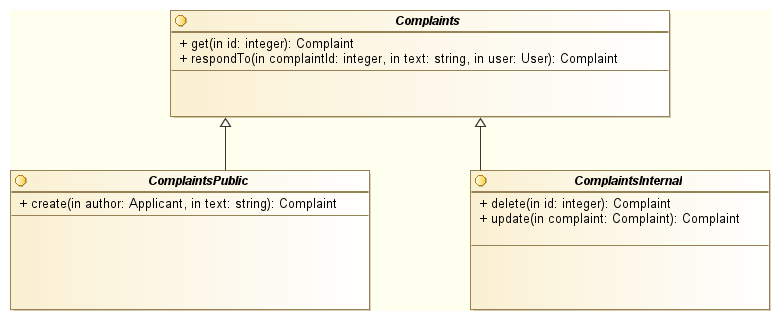
\includegraphics[scale=0.6]{uml/complaintsinterface.png}
    \caption{Erstellen der Verschiedenen Complaints Interfaces}
\end{figure}

Die verschiedenen Schnittstellen können nun in das Architekturkomponentendiagramm integriert werden. Dies wird für alle Komponenten durchgeführt und schließt die Architekturplanungsphase ab.

Nun kann mit der Implementierungsphase begonnen werden, welche sicht nicht nur mit der Technologie, sondern auch der Programmstruktur beschäftigt. Die Implementierungsphase aus Gründen des Umfangs nicht mehr Teil dieses Prozesses.

\begin{figure}[H]
    \centering
    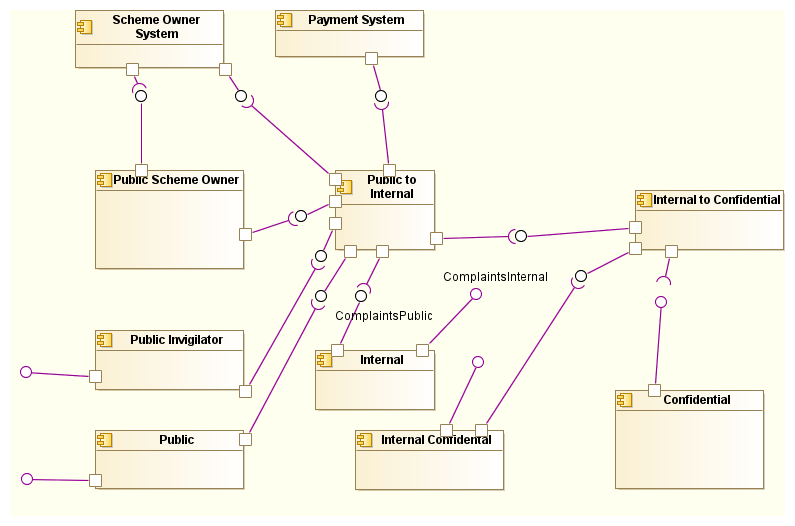
\includegraphics[scale=0.6]{uml/v5.png}
    \caption{Verlinken der Complaints Schnittstelle}
\end{figure}
\chapter{Zusammenfassung}
In der Arbeit wurde anhand eines Beispielprojektes ein UML-basierter, allgemein anwendbarer Architekturprozess erstellt, mit welchem sich reproduzierbare Softwarearchitekturen erstellen lassen. Der Architekturprozess ordent sich in die Planungsphase der Architektur ein und verwendet für die Rechtfertigung der Architekturentscheidungen einen kostenbasierten Ansatz.

Die intiale Frage - Wie kommt man von Anforderungen auf eine gute Architektur - kann wegen der ungenauen Definition einer guten Architektur nicht genau beantwortet werden. Die Frage muss anders formuliert werden, nämlich wie folgt: Wie kommt man von Anforderungen auf eine angemessene Architektur. Eine angemessene Architektur ist eine Architektur, welche die Anforderungen des/der KundIn abdeckt, nicht Mehr und nicht Weniger.

Soll nun diese Frage beantwortet werden, nämlich, ob die in der Planungsphase erstellte Architektur angemessen ist, muss die erstellte Architektur anhand von messbaren Werten überprüft und mit den gestellten Anforderungen verglichen werden. Da in der Planungsphase noch keine Implementation des Systems vorliegt, ist es jedoch für die meisten nicht funktionalen Anforderungen äußerst schwierig, sodass ein qualitätsbasierter Ansatz zu ungenaue Daten für die Basis eines Architekturprozesses liefert. Auch die Priorisierung von nicht funktionalen Anforderungen wie es von Oliver Vogel vorgeschlagen wird \cite[S. 374]{softarch} ist aufgrund ungenau ermittelbarer Parameter nicht gangbar. Ein darauf aufbauender Ansatz, welcher anhand der priorisierten Anforderungen bewertete Architekturstile \cite[S. 179]{review} auswählt ist nicht nur wegen der Priorisierung zu offen, sondern auch die Architekturstile sind noch auf einer zu abstrakten Ebene, um die wirklichen Komponenten für die Architektur zu ermitteln. Ein Versuch, die Abstraktion der Architekturstile zu verringern indem für jeden Stil fixe Komponenten ausgewählt werden, liefert auch keine eindeutige Lösung, wohl auch deswegen, weil die Komponenten auf die tatsächlichen Qualitäten überprüft werden müssten, was wegen der fehlenden Implementierung nicht möglich ist.

Da die meisten Architekturprozesse und -reviews wie ATAM die nicht funktionalen Anforderungen zur Entscheidungsfindung verwenden, ist dieses Ergebnis recht überraschend. Dies kann jedoch daran liegen, dass ATAM Architekturreviews nicht nur in der Planungsphase durchgeführt werden können. Im Bezug auf CBAM lassen sich Paralellitäten erkennen, CBAM selbst aber bietet zwar ein Reviewframework aber keinen detaillierten Architekturerstellungsprozess.

Der erstellte Prozess begnügt sich daher mit schon messbaren, bekannten bzw. vergleichbaren Werten wie zB. den Kosten, welche unter Anderem durch die Verwendung von Risikoszenarien ermittelt werden, zB. unerlaubter Zugriff auf Daten. Zusätzliche wird versucht, durch Analysen der nicht funktionalen Anforderungen der Architektur mögliche Risiken, Probleme und Parameter für die Entscheidungsfindung in der Implementationsphase zu generieren. Um die Fehlerkosten der Entscheidungen, welche auf den Analysen basieren, zu reduzieren werden architekturrelevante Parameter schon so früh wie möglich ermittelt, nämlich in der Anforderungsphase.

Eine Architektur muss jedoch nicht nur für sich selbst erstellt werden, sondern auch dem/der KundIn kommuniziert werden. Um dies zu erreichen können die kostenbasierten Entscheidungen und die UML Modelle herangezogen werden.


\section{Vorteile des erstellten Architekturprozesses}
Soll ein Architekturprozess für die Softwareentwicklung eingeführt werden, so muss dieser einen Vorteil gegenüber des Status Quo bieten. Welche Vorteile zeichnen den in der Arbeit beschriebene Architekturprozess jedoch aus?

Die Vorteile ergeben sich im Prinzip aus den treibenden Anforderungen an den Prozess und das Projekt: Der Prozess soll nachvollzieh- und reproduzierbar sein, sodass verschiedene Personen mit den gleichen Anforderungen eine identische oder zumindest stark identische Architektur erstellen. Der Fokus liegt auf der frühen Planungs- und nicht der Implementationsphase, das Projekt selbst ist ein mittelgroßes, typisches Projekt und erfordert durch dessen Anforderungen eine hohe Datensicherheit.

Daraus ergeben sich folgende Vorteile:

\begin{itemize}
  \item Gute Verständlichkeit
  \item Fokus auf Kosteneffizienz
\end{itemize}

\subsection{Gute Verständlichkeit}
Der Prozess ist aufgrund der Verwendung von UML in einer Modelliersprache dokumentiert, welche nicht nur eine große Bekanntheit und Verwendung findet, sondern auch oft im Anforderungsprozess verwendet wird. Der Architekturprozess kann damit auf dem Anforderungsprozess aufbauen und Modelle weiterentwicklen anstatt diese in komplett neue Modellierungen zu überführen. Dies hilft nicht nur bei der Kommunikation mit dem/der KundIn sondern auch mit dem Anforderungsteam: Wenn sich zB. Anforderungen ändern, können diese an den gleichen Modellen geändert werden. Die erstellten Modelle dienen zugleich auch als Dokumentation des Projektes und helfen bei der Wartung.

Zusätzlich profitiert der Prozess von den generellen Eigenschaften einer visuellen Modellierungssprache: Sie bildet das komplexe auf eine einfachere Darstellung ab und verringert die Information auf die wirklich wichtigen Bereiche. Durch die visuelle Komponente ist das Modell schneller aufnehm- und verstehbar als purer Prosatext.

Durch den Fokus auf Preis-Leistungsverhältnis ist es auch einfacher, die Probleme, Entscheidungen und Kosten dem Kunden zu kommunizieren, welcher wegen der fehlenden Vertrautheit mit dem Thema Softwarearchitektur oft die Entscheidungen und Notwendig dieses Bereiches anzweifelt \cite[S. 8-9]{softarch}. Da er mit Kostenfragen in der Regel vertraut ist, ergibt sich hier sogar eine Chance, bessere Anforderungen zu erlangen.

\subsection{Fokus auf Kosteneffizienz}
Durch den Einsatz des Prozesses in der frühen Architekturplanungsphase lassen sich hier die meisten Fehlerkosten einsparen: Nach der 10er Regel der Fehlerkosten steigen die Fehlerkosten mit dem Projektfortschritt exponentiell an. Durch die Einbeziehung von Parametern, auf welche  Architekturreviewszenarien aufbauen lassen sich auch hier im Vorfeld Kosten reduzieren: Dies betrifft nicht nur die Ermittlung der Parameter selbst, sondern auch die Möglichkeit, triviale Probleme, welche erst bei einem Architekturreview offensichtlich werden können, durch diese Anforderungen schon im Vorfeld identifizieren und beheben zu können.

Eine weitere kostensparende Eigenschaft ist, dass architekturrelevante Parameter schon in der Anforderungsphase ermittelt werden und somit die Anzahl der Kundenkontakte reduziert werden kann.

Softwarearchitekturentscheidungen sind oft ein Trade-Off: Durch konkurrierende Qualitätsanforderungen, zB. Performance und Wartbarkeit, ist es in den seltesten Fällen möglich, eine Architektur zu erstellen, welche in allen Qualitätsanforderungen brilliert. Aus diesem Grund ist es notwendig, eine bestimmte Vorgehensweise zur Erstellung, Bewertung und Entscheidung von Architekturen zu pflegen. Der Prozess bietet in dieser Hinsicht ein kostenbasiertes Entscheidungs- und Analysemodell an, mit welcher diese Entscheidungen gegenrechenbar werden. Dadurch, dass weitere Systeme nur dann erstellt werden, wenn sie einen Kostenvorteil bergen, entsteht eine kosteneffiziente und preislich angemessene Architektur.

Nicht nur tatsächliche Kosten, sondern auch Risikokosten werden im Architekturprozess mit einbezogen. Der Fokus des Prozesses liegt auf Angriffs-, Aufalls- und Änderungsszenarien, welche als Resultat des Umfeldes des Beispielprojektes gesehen werden können.

Ein weiterer Kostenvorteil ist die Möglichkeit, Anschaffungen und Architekturentscheidungen aufzuschieben, da sich der Prozess nicht auf eine physische Architektur fest legt. Die wichtigen Grundsteine, die Schnittstellen und Kommunikationswege, sind bereits geregelt, was zusätzlich eine Paralellisierung der Architekturerstellung erlaubt.


\section{Limitierungen, Probleme und Nachteile des erstellten Architekturprozesses}
Der Prozess ist zwar allgemein anwendbar, ist aber aufgrund der Herangehensweise für manche Gebiete schlechter geeignet. Die Probleme des sind vor allem in folgenden Bereiche auffindbar:

\begin{itemize}
  \item Ausgreift- und Erprobtheit
  \item Vollständigkeit
  \item Universelle Anwendbarkeit
\end{itemize}

\subsection{Ausgreift- und Erprobtheit}
Der Prozess wurde erst anhand eines einzigen Projektes erprobt und ging nicht über die Planungsphase der Architektur hinaus. Die Implementierungsphase und abschließende Überprüfung der implementierten Software wurde aus Zeit- und Umfangsgründen nicht durchgeführt. Dies führt nicht nur zu einer mangelnden Feedbackphase, in welcher Architekturprobleme während der Implementation offensichtlich werden hätten können, sondern auch zu einem zu starken Fokus auf die Domäne des Beispielprojekts.

Dies wird unter Anderem darin offensichtlich, dass der Prozess einen großen Wert auf Datensicherheit legt, welcher durch die dem Projekt zugrunde liegenden Anforderungen enstehen: Die Sicherheit und der richtige Umgang mit den Kundendaten ist eine bindende Anforderung zur Erfüllung des ISO Standards für Zertifizierungsstellen, ohne welchen das System nicht betrieben werden könnte. \cite{ISO_CERT}

Der Prozess ist somit noch unzureichend für den Einsatz in realen Projekten getestet. Vor Allem der Einsatz in unterschiedlichen Applikationsdomänen muss noch stärker geprüft werden.

\subsection{Vollständigkeit}
Die Probleme der Vollständigkeit des Prozesses sind unter Anderem eine Konsequenz der geringen Erprobtheit. Da es sehr viele unterschiedliche Risiken gibt und für unterschiedliche Projektfelder unterschiedliche Qualitäten verlangt werden, sind im Prozess nur ein Teil der möglichen Bereiche bearbeitet worden.

Außerdem behandelt der Prozess nur die Planungsphase und nicht die Architekturphase und beschäftigt sich somit weder mit der Strukturierung des Codes, noch gibt er Auskunft über die tatsächlichen eingesetzten, physischen Komponenten.


\subsection{Universelle Anwendbarkeit}
Der Architekturprozess ist vor allem geeignet für Informationssysteme, deren Fokus auf folgenden Anforderungen liegt:

\begin{itemize}
  \item Daten unterschiedlicher Vertraulichkeit müssen verarbeitet werden
  \item Datensicherheit ist wichtig
  \item Nicht jede AkteurIn kann auf alle Daten zugreifen
  \item Preis-Leistungsverhältnis ist wichtig für die Erstellung der Software
\end{itemize}

Liegt der Fokus jedoch auf anderen Bereichen, kann das Resultat der Analysen eine sehr simple Architektur sein, welche im Implementationsprozess stark angepasst werden müssen.

Ein Beispiel hierfür ist das Erstellen einer Architektur für ein sehr rechenintensives Systems, zB. für die Berechnung von Primzahlen. Hier ist es wichtig, die Berechnungen gut zu paralellisieren; der Architekturplanungsprozess würde aufgrund der Anforderungen eine einzige Softwarekomponente zur Berechnung der Primzahlen ermitteln, was zwar richtig wäre, aber wenig Hinweise zur Strukturierung der tatsächlichen physischen Systeme bieten würde.

Eine zweites Beispiel wäre ein Embedded System, welches eine starke Limitierung des Netzwerk- und Speicherdurchsatzes besitzt: Durch die Aufspaltung in mehrere Systeme, welche dann durch ein Netzwerk verbunden werden, würde die Zeit, welche zur Übermittlung der Daten aufgewendet würde stark unter der ermittelten Architektur leiden. Auch eine Virtualisierung der Komponenten auf einem System würde wegen der Speicherlimittierungen nicht in Frage kommen. Die ermittelte Architektur müsste aufgrund der Hardware Limittierungen stark überarbeitet werden.

\section{Ausblick}
Der Prozess wurde in der Planungsphase eines einzigen Beispielprojektes erprobt und schließt vor dem Beginn der Implementationsphase ab. Möglichkeiten zur Verbesserung des Prozesses lassen sich nicht nur durch die Erprobung weiterer, unterschiedlicher Projekte erlangen, sondern auch eine Erweiterung des Prozesses für die Implementationsphase ist denkbar.

Eine Möglichkeit für den Ablauf der Implementationsphase wäre folgender: Zuerst werden automatisierte Testfälle für die Qualitätsanforderungen erstellt. Die Komponentenarchitektur kann dann 1:1 auf die physische Architektur umgelegt werden, für jede Komponente wird ein physisches System eingesetzt. Die Funktionalität der Komponenten wird dann durch Prototypen umgesetzt. Anhand der Ergebnisse der Tests, wird regelmäßig überprüft, ob die geforderten Werte erreicht werden. Falls sie nicht erreicht werden, kann eine andere Architektur für die jeweilige Komponente anhand eines Prototypen überprüft werden.

Die Auswahl der Architektur, welche für die jeweilige Komponenten eingesetzt wird, obliegt den Entscheidungen der ArchitektInnnen, sprich basiert auf deren Erfahrungswerten. Auch der Einsatz von Architekturreviewmethoden wie ATAM kann hier für die Entscheidungsfindung hilfreich sein. Ob die Architektur angemessen ist, kann überdies durch die bereits erstellten, automatisierten Tests überprüft werden.





\clearpage
\bibliographystyle{gerabbrv}
\bibliography{Literatur}
\clearpage

% Das Abbildungsverzeichnis
\listoffigures
\clearpage


\phantomsection
\addcontentsline{toc}{chapter}{Abkürzungsverzeichnis}
\chapter*{Abkürzungsverzeichnis}
\begin{acronym}[XXXXX]
    \acro{VPN}[VPN]{Virtual Private Network}
\acro{IREB}[IREB]{Internation Requirements Engineering Board}
\acro{CRUD}[CRUD]{Create Read Update Delete}
\acro{ATAM}[ATAM]{Architecture Trade-off Analysis Method}
\acro{CBAM}[CBAM]{Cost Benefit Analysis Method}
\acro{ROI}[ROI]{Return of investment}
\acro{UML}[UML]{Unified Modeling Language}
\acro{RM-ODP}[RM-ODP]{Reference Model for Open Distributed Processing}
\end{acronym}
\clearpage



\end{document}
